\documentclass[a4paper,onecolumn,oneside,titlepage,11pt]{report}

\usepackage{comment}
\usepackage{fullpage}
%\usepackage[cm]{fullpage}
\usepackage[pdftex]{graphicx}
\usepackage{float}
\usepackage{tabularx}
\usepackage{listings}
\usepackage{tikz}
\usetikzlibrary{shapes,arrows,calc,fit}


\lstset{
	language=Java,
	basicstyle=\footnotesize
}

% Define block styles for flow diagrams
\tikzstyle{decision} = [diamond, draw, fill=black!20, 
    text width=4.5em, text badly centered, node distance=3cm, inner sep=0pt]
\tikzstyle{block} = [rectangle, draw, fill=black!20, 
    text width=5em, text centered, rounded corners, minimum height=4em]
\tikzstyle{highblock} = [rectangle, draw, fill=black!20, 
    text width=5em, text centered, rounded corners, minimum height=15em]
\tikzstyle{smallblock} = [rectangle, draw, fill=black!20, text centered, 
	text width=3em, rounded corners, minimum height=1em]
\tikzstyle{line} = [draw, -latex']
\tikzstyle{cloud} = [draw, ellipse,fill=red!20, node distance=3cm,
    minimum height=2em]

\def\tm{\leavevmode\hbox{$\rm {}^{TM}$}}

\definecolor{light_gray}{rgb}{0.8,0.8,0.8}

\title{Android-based Crowd Sourcing of Landmark Metadata
\\
\vspace{0.3cm}
{\normalsize github.com/alexdamian/AndroAR}}
\author{Alexandru Marian Damian}
\date{16 June 2012}

\begin{document}
\pagenumbering{roman}

\begin{comment}
\begin{titlepage}
	\begin{center}
		{\Large University POLITEHNICA of Bucharest}
		\par\vspace*{2mm}
		{\Large Faculty of Automatic Control and Computers,
		
		Computer Science and Engineering Department}
		\par\vspace*{3mm}
		\begin{table*}[h]
        	\begin{center}
				\begin{tabular}{cccc}
                    
\includegraphics[width=0.13\textwidth]{images/upb.png}
					& & &
					
\includegraphics[width=0.30\textwidth]{images/cs.png}
            	\end{tabular}
			\end{center}
		\end{table*}
		
		\par\vspace*{35mm}
		{\Huge BACHELOR THESIS}
		\par\vspace*{15mm}
		\mbox{\huge Android-based Crowd Sourcing of Landmark Metadata}\\
		\vspace{0.5cm}
		github.com/alexdamian/AndroAR\\
		\par\vspace*{35mm}
		\begin{table*}[h]
        	\begin{center}
				\begin{tabular}{lcccccl}
					\Large \textbf{\Large Scientific Advisers:}
					\vspace*{1mm} &&&&&& \Large \textbf{\Large Author:}\vspace*{1mm} \\
					\Large Prof. dr. ing. Adina Magda Florea &&&&&& \Large Alexandru Damian\\
					\Large As. drd. ing. Andrei Ismail &&&&&& \\
				\end{tabular}
			\end{center}
		\end{table*}

		\par\vspace*{38mm}
		\Large Bucharest, 2012
	\end{center}
\end{titlepage}
\end{comment}

\maketitle
\begin{abstract}
Augmented Reality has gained much interest in recent years, mostly backed by the smartphone surge, and many applications focusing on it have been created. These applications rely on sensor-generated data from inputs such as sound, video or GPS positioning. Most mobile applications rely on just a small subset of inputs (\emph{i.e. only GPS positioning data, or only the camera's video feed}).

We wanted to create an application that will help people get around unknown environments. Typical use-cases include freshmen getting around their University campuses, or tourists travelling to new cities.

At the same time, we wanted to experiment with a combination of \emph{image recognition algorithms} and \emph{GPS positioning data}, in order to achieve a high-quality user experience.

We designed and implemented an augmented reality application for Android-based smartphones which allows users to receive information about the landmarks (\emph{i.e. buildings, statues, etc.}) in their line of sight. Information is attached to bounding boxes drawn around the landmarks. Detection occurs using a combination of GPS positioning and object detection, based on the training examples we have stored in our database. These examples are generated by crowdsourcing annotated landmark data from users.

\vspace{1cm}

\textbf{Keywords}: \emph{augmented reality, image recognition, pattern recognition, object detection, live, crowdsourcing, Java, Android, Cassandra, OpenCV, database, feeds, AndroAR}
\end{abstract}
\tableofcontents

\chapter{Introduction}
\label{chap:introduction}
\setcounter{page}{1}
\pagenumbering{arabic}
\section{Motivation}
Ambient intelligence and, in particular, augmented reality are becoming increasingly popular, mainly due to the surge of smartphones and the increasing Internet connectivity options users have. Researchers and companies are offering applications that are more \textbf{interactive}, \textbf{easier to use} and better \textbf{integrated} with what the user sees and feels.

In February 2001, ISTAG (\emph{IST Advisory Group}) proposed 4 scenarios for how ambient intelligence applications will interact with users in 2010\cite{ist01}. While those scenarios are far from being implemented today, much research has been conducted in this field and numerous applications have been developed.
Two of the most recent and most interesting examples are:
\begin{enumerate}
	\item \textbf{Google Glasses}\footnote{https://plus.google.com/111626127367496192147}. This project is currently in development and plans to offer augmented reality directly in the user's line of sight, on a transparent glass cube, without them needing a smartphone or any kind of screen. The latest developments and demos have been presented at the Google IO 2012 conference (June 27 - 29). Planned features are:
	\begin{itemize}
		\item phone and video calls;
		\item video capture, along with sharing;
		\item navigation;
		\item notifications (messages, emails, calendar events);
	\end{itemize}
	\item \textbf{BMW head-up display}. BMW offers the option of augmenting information on the windshields of their high-end cars, in order for the driver to be more focused on the road ahead. Augmented information includes:
	\begin{itemize}
		\item current speed, gear, etc.
		\item turn-by-turn navigation;
		\item speed limitations, radars;
		\item car notifications.
	\end{itemize}
\end{enumerate}
However, most applications currently tend to pivot around \emph{just} one of the two most common ideas:
\begin{enumerate}
	\item augmenting different layers of information (\emph{i.e. social-media information -- friends' checkins, tweets, Facebook posts, Google+ posts --, tourist information -- hotels, restaurants, parks, museums --, even historical events -- wikipedia articles --}) mainly based on GPS positioning;
	\item augmenting information based on a snapshot of what the user sees (\emph{i.e. a frame in the phone's camera feed}).
\end{enumerate}
The use-cases we must to deal with will force us to implement a mixture of the two ideas stated above.

\section{Proposed Application -- AndroAR}
We propose a mobile application called AndroAR that will augment landmark information on the current camera feed. Queries containing the camera frame, GPS position, orientation and other sensor data will be sent to a server. It will retrieve, from a database, all the possible landmarks that can appear in the received camera frame, and will forward their instances (\emph{i.e. images}) to an image recognition component, which will decide if they are present or not in the frame. Metadata for these objects will be returned to the user's mobile application, in order to be augmented on the screen.

Our application will support and will encourage crowdsourced contributions to annotate landmarks. We will offer a way for the user to freeze the camera feed on a particular frame, crop a landmark and annotate it with metadata. We will also be using different techniques to passively generate additional correct instances of objects that have already been annotated.

An example use-case of our application is: a tourist is travelling to a foreign country and uses AndroAR to find his way around an unknown city. Information about landmarks \emph{that he sees} will be augmented in the application, on top of the camera feed.

We would like to thank Andrei Petre\footnote{student at the Polytechnic University of Bucharest, Faculty of Automatic Control and Computers, second year} for developing the Android application.
\section{Structure of Thesis}
The structure of this thesis is as follows:
\begin{itemize}
	\item chapter \ref{chap:introduction} presents the motivation for choosing this subject;
	\item chapter \ref{chap:state-of-the-art} offers information regarding the most widely used and most innovative augmented reality applications;
	\item chapters \ref{chap:goals}, \ref{chap:system-design} and \ref{chap:system-workflow} present the goals for our application, the design and the workflow of our system;
	\item chapter \ref{chap:performance-issues} presents the problems that arise given the system design and the goals of our application;
	\item chapter \ref{chap:implementation} presents details regarding the  implementation of this system;
	\item chapters \ref{chap:results} and \ref{chap:conclusions} present the results, conclusions and future work.
\end{itemize}

\chapter{State of the Art}
\label{chap:state-of-the-art}
Augmented reality is very popular in the mobile industry. However, most applications interact very little with the video feed they overlay the information on. Typically, applications will:
\begin{itemize}
	\item interact with a small part of the current view, such as a \emph{logo} or \emph{banner};
	\item take advantage of the localization capabilities of the phone, such as \emph{GPS positioning} or \emph{compass}, but place information on the screen with disregard to what the user's line of sight actually is (\emph{e.g. a user might be facing a wall and be overrun with information, even though he doesn't see anything relevant}).
\end{itemize}
We will present the most popular and most innovative products that currently exist on the market, also stating what their disadvantages are \emph{relative to} the implementation of our application's use-cases.
\section{Layar}
Layar\footnote{http://www.layar.com/} is a mobile application built for Android and iOS. It is the most well-known augmented reality mobile application in the industry. Having pivoted a few times, it now focuses on bringing the augmented reality experience to printed publications.

\textbf{However}, Layar's current focus makes it unsuitable. One can try to associate a current view of the world (\emph{i.e. what the user sees at a particular moment through the smartphone's camera}) with a \emph{printed magazine page}. But the world is dynamic and tridimensional, and, therefore, problems will arise when trying to extend the Layar behavior.

We must note that Layar has limited support for displaying 3D objects.
\section{Google Maps / Street View}
Google Maps\footnote{http://maps.google.com/} enables users to navigate and receive directions on an extremely detailed map. Street View, a subproduct of Google Maps, offers navigation at street level, allowing the user to asociate information with their surroundings.

\begin{figure}[H]
\begin{center}
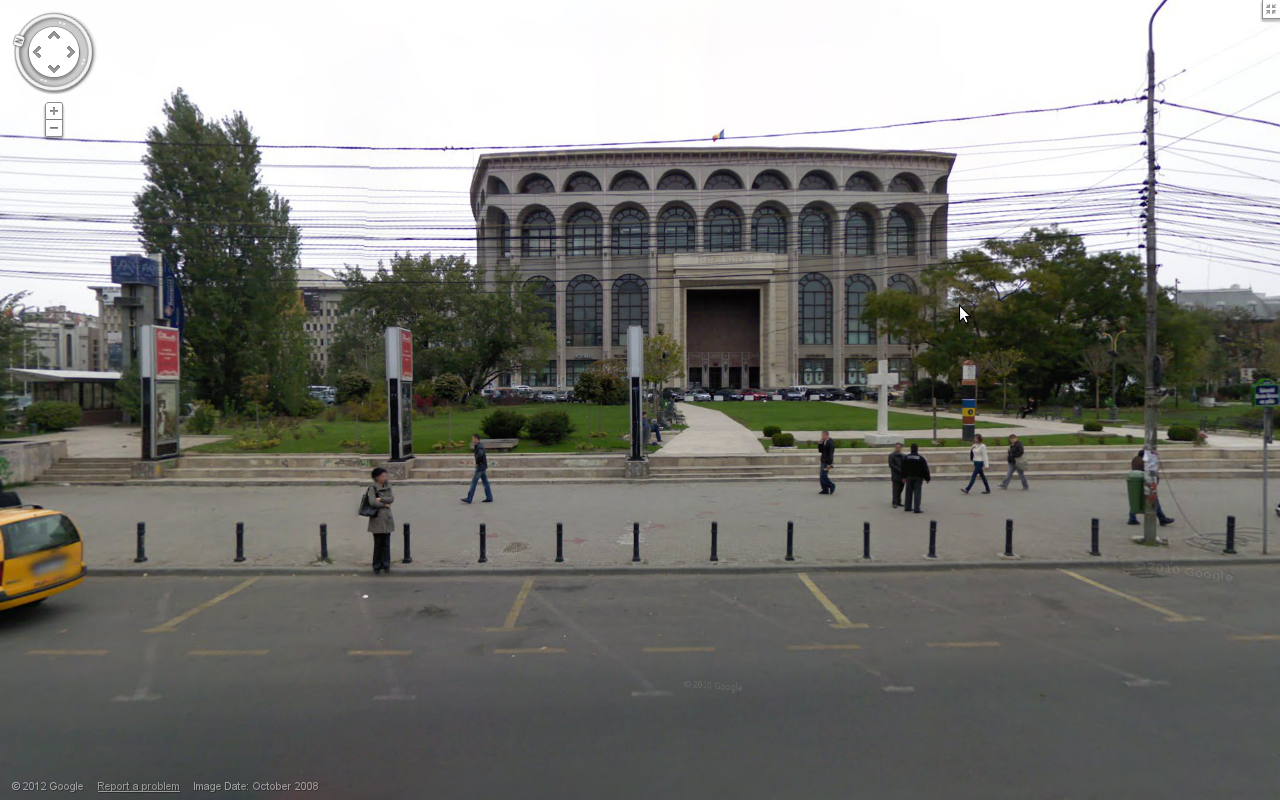
\includegraphics[width=8cm]{images/tnb_streetview.png}
\caption{Screen caption of the Street View web application}
\end{center}
\end{figure}

\textbf{However},
\begin{itemize}
	\item Street View is not live. Street View imagery was captured using dedicated equipment. Efforts are being made to keep the imagery as up-to-date as possible, but this can not be done all around the world. For example, several areas in Romania contain images that are 4 years old.
	\item only recently has Street View begun offering imagery outside of street range (\emph{i.e. pedestrian roads, parks, campuses, indoor}).
	\item users can navigate through Street View using their smartphone, but the Street View imagery will completely replace what the user sees.
\end{itemize}
\section{Wikitude}

Wikitude\footnote{http://www.wikitude.com/} is one of the first implementations of an augmented reality environment. Wikitude is more feature-rich than Layar, offering more than $3500$ so-called \emph{worlds} (which are, basically, layers of information that will be displayed on top of the current camera feed, \emph{i.e. tweets, nearby hotels, events, etc.}). One of the most interesting aspects of it is that it offers a SDK for development of new features.

\begin{figure}[H]
\begin{center}
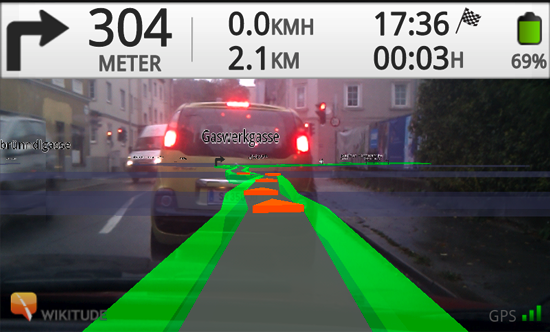
\includegraphics[width=8cm]{images/wikitude_drive.png}
\caption{Screen caption of the Wikitude Drive application}
\end{center}
\end{figure}

\textbf{However}, even though there are many sources of information that can be presented to the user, \emph{Wikitude} still doesn't take advantage of what the user actually sees, but only their position and orientation.

We must note that an application called \textbf{Wikitude Drive} exists, offering \emph{turn-by-turn navigation}, augmented over the current view of the road.

\chapter{Goals for AndroAR}
\label{chap:goals}
AndroAR is designed to offer a \emph{true} augmented reality experience, by interleaving the \emph{localization features} with \emph{image recognition} algorithms. While designing AndroAR, we focused on several requirements, which we will present below, along with reasons why the current solutions can not be used or are difficult to extend.
\section*{Live}
We need to focus on displaying information relevant to what the user sees, not just to the user's position and orientation. Most augmented reality applications will place an overlay of information on top of the current camera feed; the two are related only by the current localization features of the user (\emph{i.e. GPS position, compass orientation}) and not by what the camera feed actually shows.

A typical example in which such applications perform poorly is when two buildings are collinear and viewed from an angle such that the second one is fully covered by the first one. Most applications will offer information related to both buildings, even if the user can only see one. Although this can be solved by testing for collinearity, there is no solution when the covering object is not annotated, or if it is temporary located there (\emph{i.e. mobile advertising panel}).

\textbf{Layar} offers a live view, but is only focused on paper.

\textbf{Street View} doesn't offer a live view, but Google Maps supports uploading of user images and tagging; these images can be augmented onto the Street View imagery, but that only works on the desktop web version.

\begin{figure}[H]
\begin{center}
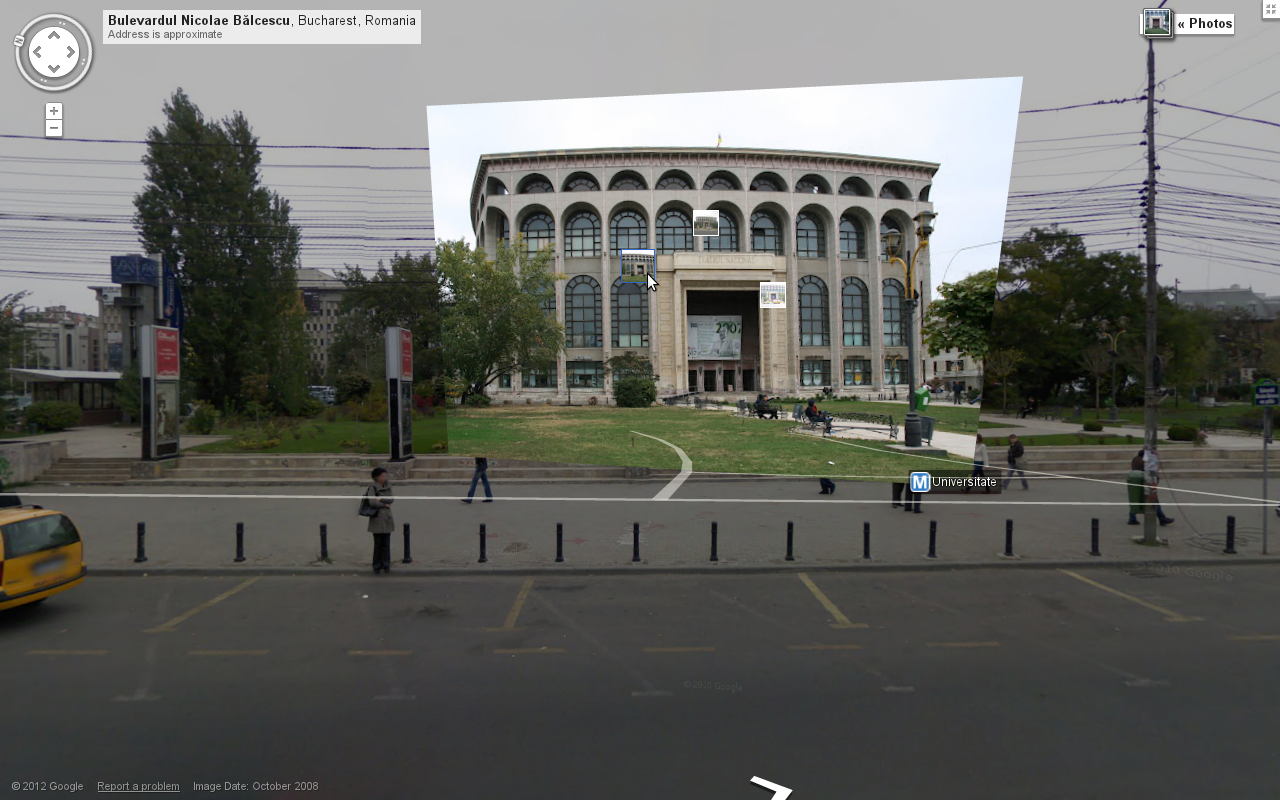
\includegraphics[width=7.9cm]{images/streetview_augmentation.png}
\caption{Example of augmentation of a user-submitted photo in Street View}
\end{center}
\end{figure}

\textbf{Wikitude} is live and shows information originating in an area around the user. We can use their SDK to retrieve the subset of objects around the user's current position and then use our own algorithms to select which objects' information to display. But even so, we must deal with aquiring the data (either by user input, or by crawling different sources that have the mapping \emph{object information} $\rightarrow$ \emph{object image} available) and storing it in a Wikitude-friendly way.
\section*{Latency}
Using the camera feed brings up some issues regarding speed and bandwidth since displaying information is not a matter of only querying a database with the user's current position anymore. We need to find a way to divide the computational effort between the server and the mobile application. We must also consider the effect of latency on the query replies (\emph{i.e. by the time the user receives the query reply, the detected objects might have translated).}

By its design, \textbf{Layar} users are expected to wait for the reply to the query. A typical usecase of Layar is: \emph{a user will see the message \emph{Scan for a making-of video} on the cover of a magazine and will wait for the application to serve the video}.

Since it's not live, \textbf{Street View} can precache the information it needs in order to serve information to the user. By its design, Street View queries will not be affected by what the users see, but only by their position.

\textbf{Wikitude} will definitely have a speed advantage over our application, since they involve only querying a database and not executing any other CPU-intensive operations (\emph{i.e. image recognition}).

\section*{Correct}
We must make sure that the information (\emph{i.e. objects associated with images and metadata}) is correct. Since we are using a crowdsourced approach, we should consider rating of images to allow removal of incorrect associations. Also, we must deal with spam.

\textbf{Layar} has fewer problems with this since they are using a business-to-consumer model, in which the information is provided by the business and the queries are made by the consumer (\emph{i.e. a magazine creates the layers and the reader uses the application}). Layar can correctly assume that businesses will provide high-quality information.

\textbf{Street View} already has correct and high-quality imagery. Images added by users can be easily filtered by first querying them against the existent database.

Information available in \textbf{Wikitude} has a very high probability of being correct, since it is backed by a community, but we are interested in \emph{object information} $\rightarrow$ \emph{object image} associations, and Wikitude contains \emph{object information} $\rightarrow$ \emph{object localization} associations.

\chapter{System Design}
\label{chap:system-design}
The basic design of the system has 5 components:
\begin{enumerate}
	\item server,
	\item storage,
	\item image recognition component,
	\item mobile application,
	\item communication layer,
\end{enumerate}
connected as follows:

\begin{figure}[H]
\begin{center}
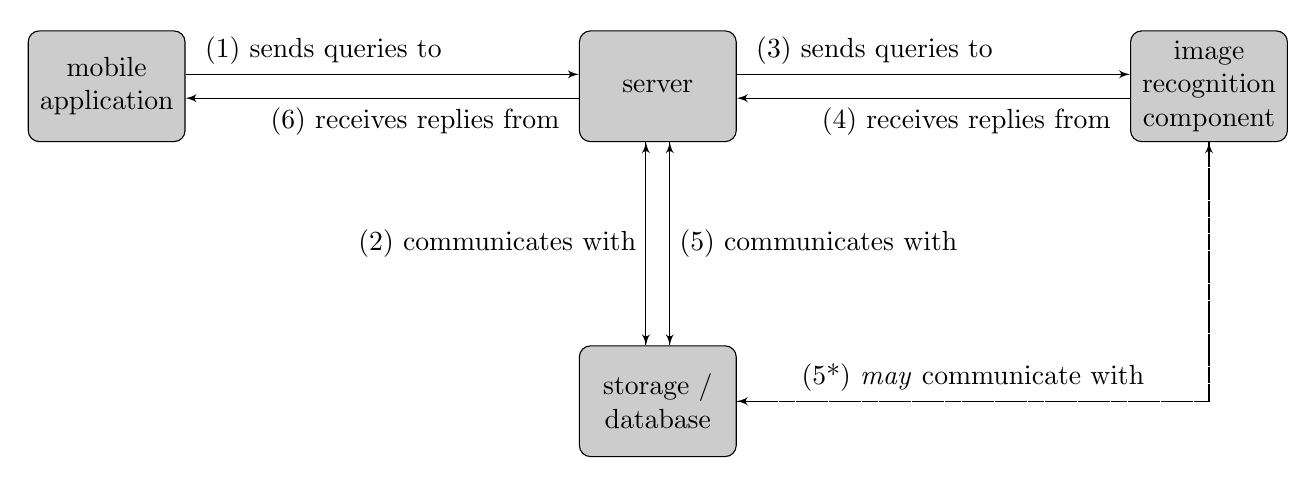
\begin{tikzpicture}[node distance = 2cm, auto]
    % Place nodes
    \node [block] (app) {mobile application};
    \node [block, right of=app, node distance=7cm] (server) {server};
    \node [block, below of=server, node distance=4cm] (db) {storage / database};
    \node [block, right of=server, node distance=7cm] (ai) {image recognition component};
    % Draw edges
    \path [line] ([yshift=1ex] app.east) -- node [above, text width=4.5cm, align=left] {(1) sends queries to} ([yshift=1ex] server.west);
    \path [line] ([yshift=-1ex] server.west) -- node [below, text width=4.5cm, align=right] {(6) receives replies from} ([yshift=-1ex] app.east);
    \path [line] ([yshift=1ex] server.east) -- node [above, text width=4.5cm, align=left] {(3) sends queries to} ([yshift=1ex] ai.west);
    \path [line] ([yshift=-1ex] ai.west) -- node [below, text width=4.5cm, align=right] {(4) receives replies from} ([yshift=-1ex] server.east);    
    \path [line] ([xshift=-1ex] server.south) -- node [left, text width=4cm, align=right] {(2) communicates with} ([xshift=-1ex] db.north);
    \path [line] ([xshift=-1ex] db.north) -- ([xshift=-1ex] server.south);  
    \path [line] ([xshift=1ex] server.south) -- node [right, text width=4cm, align=left] {(5) communicates with} ([xshift=1ex] db.north);
    \path [line] ([xshift=1ex] db.north) -- ([xshift=1ex] server.south);
    \path [line, dashed] (ai) |- (db);
    \path [line, dashed] (db) -| node [near start] {(5*) \emph{may} communicate with} (ai);
\end{tikzpicture}
\end{center}
\caption{Basic system design}
\end{figure}
Note that, although \emph{arrows (2)} and \emph{(5)} both share the same caption, the transferred messages they refer to are different:
\begin{itemize}
	\item \emph{arrow (2)} refers to messages related to queries that are received by the \emph{server} from the \emph{mobile application}. These messages will aid the server in preparing the more complex query that will be sent to the \emph{image recognition component};
	\item \emph{arrow (5)} refers to messages related to queries and replies that are received by the \emph{server} after being parsed by the \emph{image recognition component}.
\end{itemize}
The system design can be easily scaled, by implementing one of the following:
\begin{enumerate}
	\item \emph{Servers}, \emph{image recognition components} and \emph{database instances} are selected from different pools.

\begin{figure}[H]
\begin{center}
\begin{tikzpicture}[node distance = 2cm, auto]
    % Place nodes
    \node [block] (app) {mobile application};
    \node [block, right of=app, node distance=3cm, text width=2cm] (server) 
    {
    	\begin{tikzpicture}
    		\node [smallblock] (server1) {S 1};
    		\node [smallblock, below of=server1, node distance=1cm] (server2) {S 2};
    	\end{tikzpicture}
    	
    	$\vdots$
    	\vspace{2mm}
    	
    	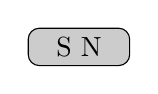
\begin{tikzpicture}
    		\node [smallblock] (servern) {S N};
    	\end{tikzpicture}
    };
    \node [block, right of=server, node distance=3cm, text width=2cm] (ai) 
    {
    	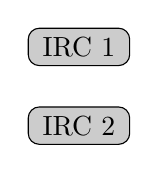
\begin{tikzpicture}
    		\node [smallblock, node distance=2cm] (ai1) {IRC 1};
      		\node [smallblock, below of=ai1, node distance=1cm] (ai2) {IRC 2};
    	\end{tikzpicture}
    	
    	$\vdots$
    	\vspace{2mm}
    	
    	\begin{tikzpicture}
    		\node [smallblock, below of=ai1, node distance=2cm] (ain) {IRC N};
    	\end{tikzpicture}
    };
    \node [block, right of=ai, node distance=3cm] (db)
    {
        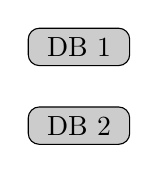
\begin{tikzpicture}
    		\node [smallblock] (db1) {DB 1};
    		\node [smallblock, below of=db1, node distance=1cm] (db2) {DB 2};
    	\end{tikzpicture}
    	
    	$\vdots$
    	\vspace{2mm}
    	
    	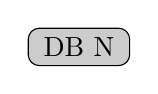
\begin{tikzpicture}
    		\node [smallblock] (dbn) {DB N};
    	\end{tikzpicture}
    };
    % Draw edges
    \path [line] (app) -- (server);
    \path [line] (server) -- (app);
    \path [line] (server) -- (ai);
    \path [line] (ai) -- (server);
    \path [line] (ai) -- (db);
    \path [line] (db) -- (ai);
    \path [line] (server.south) -- +(0.0, -0.5) -- +(+6, -0.5) -- node [above, midway] {} (db.south);
    \path [line] (db.south) -- +(0.0, -0.5) -- +(-6, -0.5) -- node [above, midway] {} (server.south);
\end{tikzpicture}
\end{center}
\caption{Design option for scaling the system, using \emph{3} pools for \emph{servers}, \emph{image recognition components} and \emph{databases}}.
\end{figure}
	\item Each \emph{server} is associated with its own \emph{image recognition component}. The \emph{server + image recognition component} and the \emph{database} are chosen from their respective pools. Each time an \emph{image recognition component} needs to query the database, it will forward the request to the \emph{server}, which will act as a \emph{transit component}, therefore reducing the implementation time, while still keeping high performance.
	
\begin{figure}[H]
\begin{center}
\begin{tikzpicture}[node distance = 2cm, auto]
    % Place nodes
    \node [block] (app) {mobile application};
    \node [block, right of=app, node distance=4cm, text width=4cm] (server) 
    {
    	\begin{tikzpicture}
    		\node [smallblock] (server1) {S 1};
    		\node [smallblock, right of=server1, node distance=2cm] (ai1) {IRC 1};
    		\node [smallblock, below of=server1, node distance=1cm] (server2) {S 2};
      		\node [smallblock, right of=server2, node distance=2cm] (ai2) {IRC 2};
      		
      		\path [line] (server1) -- (ai1);
      		\path [line] (ai1) -- (server1);
      		\path [line] (server2) -- (ai2);
      		\path [line] (ai2) -- (server2);
    	\end{tikzpicture}
    	
    	$\vdots$
    	\vspace{2mm}
    	
    	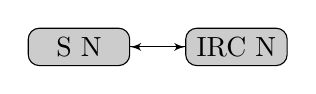
\begin{tikzpicture}
    		\node [smallblock] (servern) {S N};
    		\node [smallblock, right of=servern, node distance=2cm] (ain) {IRC N};
    		\path [line] (servern) -- (ain);
      		\path [line] (ain) -- (servern);
    	\end{tikzpicture}
    };
    \node [block, right of=server, node distance=4cm] (db)
    {
        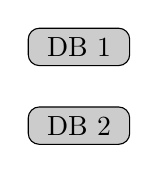
\begin{tikzpicture}
    		\node [smallblock] (db1) {DB 1};
    		\node [smallblock, below of=db1, node distance=1cm] (db2) {DB 2};
    	\end{tikzpicture}
    	
    	$\vdots$
    	\vspace{2mm}
    	
    	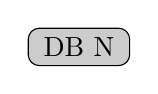
\begin{tikzpicture}
    		\node [smallblock] (dbn) {DB N};
    	\end{tikzpicture}
    };
    % Draw edges
    \path [line] (app) -- (server);
    \path [line] (server) -- (app);
    \path [line] (server) -- (db);
    \path [line] (db) -- (server);
\end{tikzpicture}
\end{center}
\caption{Design option for scaling the system, with each \emph{server} being connected to the corresponding \emph{image recognition component}, therefore using only \emph{2} pools.}
\end{figure}
\end{enumerate}
When scaling the system, we must take into account several aspects:
\begin{enumerate}
	\item the state of the system is completely stored in the \emph{database}. The \emph{server} and the \emph{image recognition component} are stateless and can therefore be easily scaled, by using more instances;
	\item the \emph{database} is stateful and is, therefore, more difficult to scale. Also, we must take into account the high number of writes our database must accomodate.
	
	For example, \emph{Netflix} has chosen \textbf{Apache Cassandra} as the database for their system. Experiments conducted by them showed excellent performance under high amounts of write requests, achieving 1.1 million writes per second (or 3.3 million writes per second after replication with a factor of $3$) when using a cluster of 96 medium sized Amazon EC2 instances (or 288, after replication)\footnote{http://techblog.netflix.com/2011/11/benchmarking-cassandra-scalability-on.html}.
\end{enumerate}

\chapter{Information Flow Through the System}
\label{chap:system-workflow}
A user can interact with our application in two ways:
\begin{enumerate}
	\item by making queries while using the application;
	\item by sending images annotated with objects and metadata.
\end{enumerate}
We will illustrate the overall workflow for each of them below.

\section{Queries}
Let us assume that at one point in time, while the user is using the application, it needs to find all the objects that appear in a frame, along with their metadata. To accomplish this, we will send a request to the server that will be completed in the following steps:
\begin{enumerate}
	\item The mobile application will encapsulate the current frame, along with localization information (GPS position and compass orientation) and send it to the server;
	\item The server will forward the query to the database which will fetch from storage, all the possible objects in the user's line of sight. We define the user's \emph{line of sight} as a \emph{cone} in front of the user, as shown below. All the objects that are in the user's line of sight are marked in \emph{green}. The objects that we consider as being not observable are marked in \emph{red}:

\begin{figure}[H]
\begin{center}
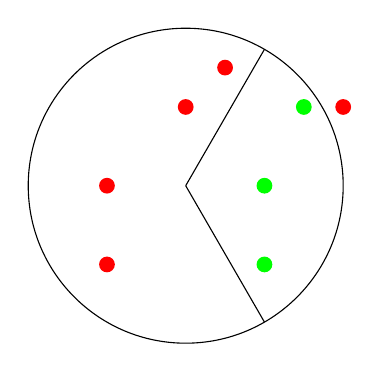
\begin{tikzpicture}
	\draw (0, 0) circle (2cm);
	\draw (0, 0) -- +(-60:2cm);
	\draw (0, 0) -- +(60:2cm);
	
	\newcounter{i}
	\setcounter{i}{0}
	\foreach \point in
	{(1,0),(1.5, 1), (1, -1)}
	{
    	\node[coordinate] (point-\arabic{i}) at \point { };
    	\fill [color=green] (point-\arabic{i}) circle (0.1);
    	\stepcounter{i}
	}
	\setcounter{i}{0}
	\foreach \point in
	{(-1, 0),(-1,-1),(0,1), (0.5, 1.5), (2,1)}
	{
    	\node[coordinate] (point-\arabic{i}) at \point { };
    	\fill [color=red] (point-\arabic{i}) circle (0.1);
    	\stepcounter{i}
	}
\end{tikzpicture}
\end{center}
\caption{Example of using the line of sight to retrieve a subset of possible matches}
\end{figure}
	
	\item The database will return the objects that might pe present in the frame. For each object, information that will help match the particular object to an image will also be returned. Note that each object may (and should) be present in more than one image. We will return matching information for the best performing subset of these images, which may contain:
	\begin{enumerate}
		\item image features (\emph{e.g. lines, corners, areas of constrast, etc.});
		\item illumination information;
		\item etc.
	\end{enumerate}
	\item We will forward the initial query, along with the possible objects to the image recognition component. This component will:
		\begin{enumerate}
			\item compute the features for the query image;
			\item compare the features for the query image to the features of every possible object and assign a rate of success (or certainty) to each statement
			
			$X$ is present in the query image $I$, where $X$ is a $possible\:object$
		\end{enumerate}
		\item Using a threshold for the rate of success, we will end up with a subset of the possible objects being classified as detected objects. These detected objects, along with the corresponding positions in the query image, will be sent back to the server by the image recognition component.
		\item The server will then forward the reply to the mobile application.
\end{enumerate}

\begin{figure}[H]
\begin{center}
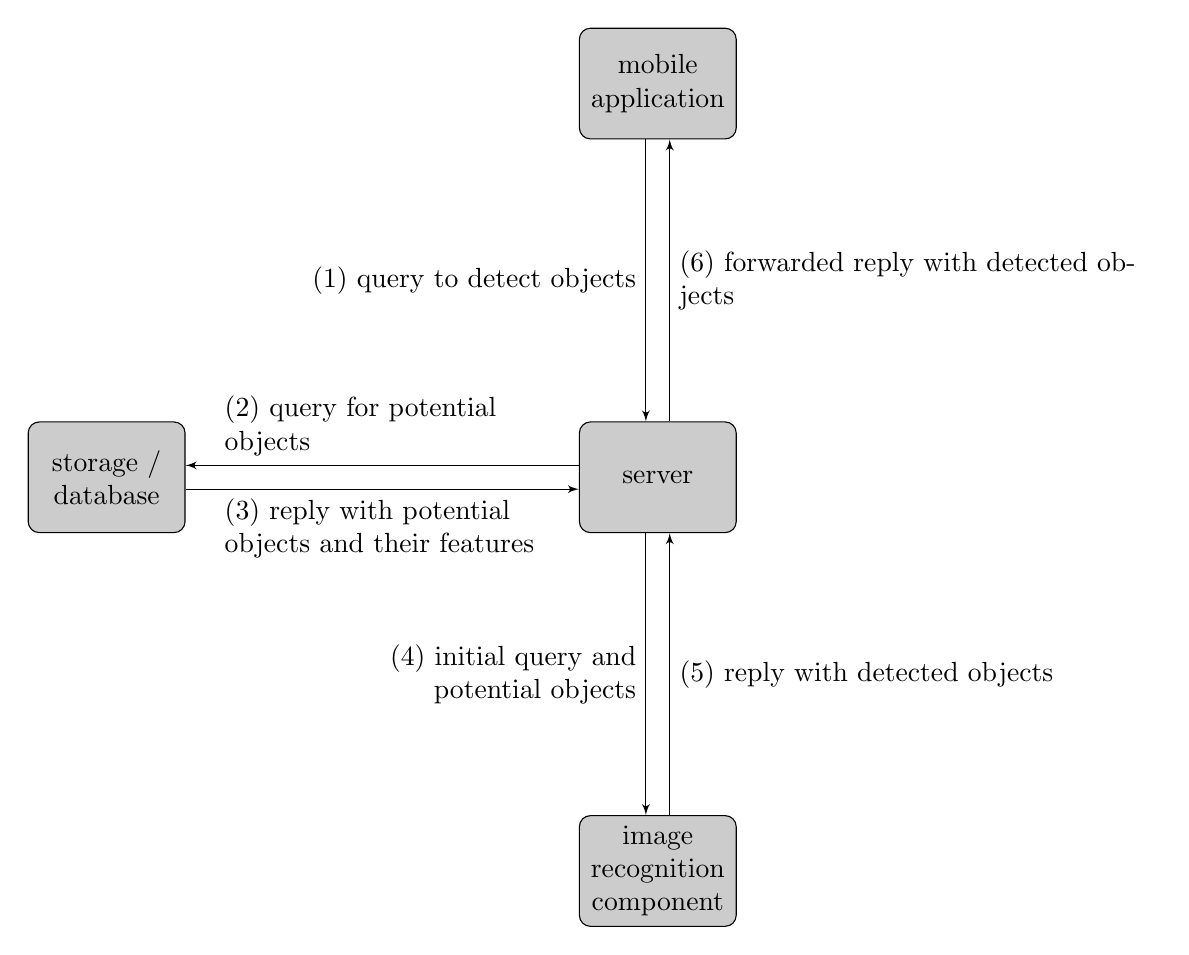
\begin{tikzpicture}[node distance = 2cm, auto]
    % Place nodes
    \node [block] (app) {mobile application};
    \node [block, below of=app, node distance=5cm] (server) {server};
    \node [block, left of=server, node distance=7cm] (db) {storage / database};
    \node [block, below of=server, node distance=5cm] (ai) {image recognition component};
    % Draw edges
    \path [line] ([xshift=-1ex]app.south) -- node [left, text width=5cm, align=right] {(1) query to detect objects} ([xshift=-1ex]server.north);
    \path [line] ([yshift=1ex]server.west) -- node [above, text width=4cm] {(2) query for potential objects} ([yshift=1ex]db.east);
    \path [line] ([yshift=-1ex]db.east) -- node [below, text width=4cm] {(3) reply with potential objects and their features} ([yshift=-1ex]server.west);
    \path [line] ([xshift=-1ex]server.south) -- node [left, text width=4cm, align=right] {(4) initial query and potential objects} ([xshift=-1ex]ai.north);
    \path [line] ([xshift=1ex]ai.north) -- node [right, text width=6cm] {(5) reply with detected objects} ([xshift=1ex]server.south);
    \path [line] ([xshift=1ex]server.north) -- node [right, text width=6cm] {(6) forwarded reply with detected objects} ([xshift=1ex]app.south);
\end{tikzpicture}
\end{center}
\caption{Life of a query.}
\end{figure}
\subsection*{Example}
We will illustrate the previous workflow with an example:
\begin{itemize}
	\item Let us assume that a tourist is travelling through Paris and, when a query is made to the server, he is looking at the \emph{Eiffel Tower}.
	\item The server will receive a query containing an image of the \emph{Eiffel Tower}, along with the tourist's position and orientation. 
	\item The server will then request, from the database, all the possible objects that might be present in the tourist's line of sight. For example, the server might request the top (at most) 10 ranking instances of all the objects in a 100 meter radius and in a 90$^\circ$ cone in front of the user.
	\item A possible reply from the server contains the features for 10 images of the \emph{Eiffel Tower} and the features for 6 images of \emph{Les Invalides}.
	\item These will be forwarded to the image recognition component which will try to match 2 possible objects with the query image. The confidence rates that result can be:
		\begin{center}
			\begin{tabular}{|c|c|}
				\hline
				\textbf{Object} & \textbf{Confidence}\\
				\hline
				Eiffel Tower & .85\\
				Les Invalides & .5\\
				\hline
			\end{tabular}
		\end{center}
	\item With a threshold of $.75$, only the \emph{Eiffel Tower} will be selected as a valid match and will be returned as the query reply.
\end{itemize}

\section{Store Requests}
Our application supports and encourages crowdsourced contributions to annotate new landmarks. Should a user want to annotate a landmark, the application will allow them to freeze on a particular camera frame, create  bounding boxes around landmarks and annotate them with information. We will need to store this information into our database.

To accomplish this, we will send a request to the server that will be completed in the following steps:
\begin{enumerate}
	\item The mobile application will encapsulate the current frame, along with localization information (GPS position and compass orientation), and the bounding boxes and metadata for each input object; it will then send this request to the server.
	\item The server will forward the request to the database, which will store the data (\emph{i.e. image, localization, objects ids, objects metadata, cropped objects images, etc.}).
	\item The server will then forward the request to the image recognition component which will compute the features for:
	\begin{itemize}
		\item the large image;
		\item the small images (\emph{i.e. images cropped according to the provided bounding boxes for the detected objects}).
	\end{itemize}
	\item The image recognition component will then send the features back to the server.
	\item The server will forward them to the database, which will store them.
\end{enumerate}

\begin{figure}[H]
\begin{center}
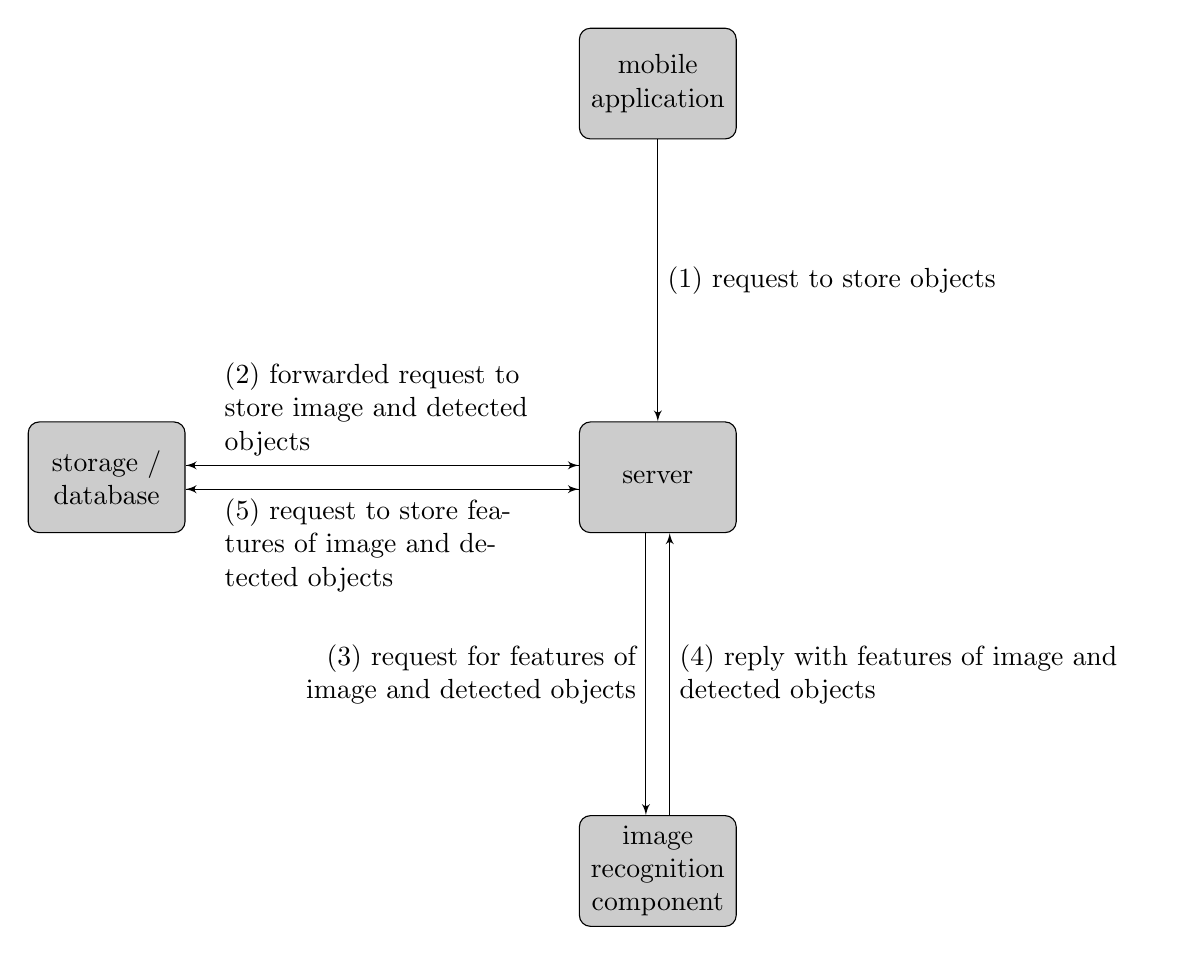
\begin{tikzpicture}[node distance = 2cm, auto]
    % Place nodes
    \node [block] (app) {mobile application};
    \node [block, below of=app, node distance=5cm] (server) {server};
    \node [block, left of=server, node distance=7cm] (db) {storage / database};
    \node [block, below of=server, node distance=5cm] (ai) {image recognition component};
    % Draw edges
    \path [line] (app) -- node [text width=6cm] {(1) request to store objects} (server);
    \path [line] ([yshift=1ex]server.west) -- node [above, text width=4cm] {(2) forwarded request to store image and detected objects} ([yshift=1ex]db.east);
    \path [line] ([yshift=1ex]db.east) -- ([yshift=1ex]server.west);
    \path [line] ([xshift=-1ex]server.south) -- node [left, text width=6cm, align=right] {(3) request for features of image and detected objects} ([xshift=-1ex]ai.north);
    \path [line] ([xshift=1ex]ai.north) -- node [right, text width=6cm] {(4) reply with features of image and detected objects} ([xshift=1ex]server.south);
    \path [line] ([yshift=-1ex]server.west) -- node [below, text width=4cm] {(5) request to store features of image and detected objects} ([yshift=-1ex]db.east);   
    \path [line] ([yshift=-1ex]db.east) -- ([yshift=-1ex]server.west);
\end{tikzpicture}
\end{center}
\caption{Life of a storage request.}
\end{figure}
\subsection*{Example}
We will illustrate the previous workflow with an example:

\begin{itemize}
	\item Let us assume that the same tourist has now arrived home, in Romania. He now wants to use the application in Bucharest, but sees that very few buildings are tagged. Even when he is pointing his smartphone at the \emph{National Theatre} building, he sees that no information is being displayed. He decides to annotate this building with metadata.
	\item He clicks on the \emph{Capture} button and the camera feed freezes on the current frame. He must then select the building by positioning and resizing a bounding box over it and insert the landmark's name and description.
	\item The server will receive a store request containing the image of the \emph{National Theatre} and its surroundings, a cropped image of the \emph{National Theatre}, metadata (name, description) and the tourist's position and orientation. 
	\item The server will then forward the request to the database, which will store all the information.
	\item Additionally, the server will request all features to be computed for both the original image and all the smaller, cropped images. The server will then forward this information to the database to be stored accordingly.
\end{itemize}
This example only illustrates basic functionality of the \emph{Storage} component. A more likely workflow is:
\begin{itemize}
	\item compute all the frames in a predefined range before and after the current frame that contain the tagged objects;
	\item detect the object's translation in order to automatically adjust the bounding box in each frame;
	\item send each frame, along with its cropped images, metadata and localization information to the server, when the mobile phone connects to a WiFi link.
\end{itemize}
We will explain ideas for capturing additional valid examples (\emph{i.e. correct object instances}) in chapter \ref{chap:performance-issues}.


\chapter{Performance Issues}
\label{chap:performance-issues}
The workflows presented in chapter~\ref{chap:system-workflow} pose several performance issues.
\section{Query Issues}
Ideally, we would want to answer queries at a rate equal to the \emph{fps} value of the current video feed. A sufficient value for the \emph{fps} would be $5-10$. We do not need the performance of a higher \emph{fps} value (\emph{i.e. the cinematic value of 24}).

However, even intuitively, it will be extremely difficult to answer queries at a rate of $5-10$ \emph{fps}, for \emph{each} connected client. Moreover, we must consider the limited amount of traffic a mobile phone has available on 3G / 4G networks. With this in mind, we should limit the amount of queries issued by the client.

\subsection{Sparse Queries}
We can achieve a good trade-off between quality and performance by using a simple observation: \emph{in most scenarios, a detected building will not disappear from the user's line of sight in less than $1-2$ seconds}; that is because the user will not pan the camera fast enough so that the entire landscape changes.

We can take advantage of this by:
\begin{enumerate}
	\item issuing sparse queries (\emph{i.e. a query every 5 seconds});
	\item in between these queries, using the orientation (mainly) and the GPS position of the device to translate or scale the bounding boxes accordingly;
\end{enumerate}
We should note that:
\begin{enumerate}
	\item there will be a delay between the moment when the query is issued and the moment when the response is received; we should translate and scale the bounding boxes according to the relative move of the device;
	\item translation and scaling according to localization capabilities will allow for higher quality user experience; let us imagine that the user is looking at a building for which the right half is very rich in features and the left side is very poor in features, and that the building is correctly detected. Should the user pan the camera to the left and have only the left half of the building visible, in the $5$ second range, a bounding box will still be shown around the building, even if the image recognition component can not further detect it.
\end{enumerate}
We will also ilustrate this in chapter~\ref{chap:implementation}, but it important to note why we chose the $5$ second range. Using a simple implementation with the following features:
\begin{itemize}
	\item \emph{SURF} detector\footnote{Speeded Up Robust Feature detector};
	\item \emph{Brute-force} matcher;
	\item 2 potential objects (totalling 4 instances), 
\end{itemize}
the average round-trip time for a query was $3.5$ seconds, using a \emph{high-quality, color, 8 megapixel} image.

\subsection{Caching}
Given that the users will change their GPS position so sightly every-time a query is issued (\emph{i.e. a typical user will travel by foot; assuming their average speed is $4 km/h$, they will travel $1$ meter every second}), we can take full advantage of \emph{caching}. We could query the database for \emph{all} the objects surrounding  the users, not just those in their cone of sight and cache their features. Should the user move, we only need to query the database for the objects in the areas previously not covered.

\section{Storage issues}

As stated above, we are using a crowdsourced approach to getting new data. However, this is often not enough, since most of the users will submit very little information.

\subsection{Passive example generation}

We have come up with some ideas to increase the number of correct examples (\emph{i.e. object instances}) that are saved to our database:
\begin{enumerate}
	\item when a user freezes on a frame and tags several objects, we can safely assume that some frames before and some frames after will also contain that object. We can therefore send them in a batch to the server to store in the database. The server should decide which of them it should keep (\emph{i.e. frames that actually contain the object and have good quality, and are not repetitive});
	\item when a mobile application instance issues a query and a reply that contains objects rated with high confidence is returned, than we can also assume that some frames before and some frames after will also contain those objects. We can then proceed as above.
\end{enumerate}

\section{Write estimations}
We must also take into account the amount of writing that needs to be supported by the database: assuming \emph{50 concurrent clients}, all with a framerate of \emph{10 fps}, each frame being sent to the servers as a \emph{800 $\times$ 600 JPEG image} of size roughly \emph{300 kilobytes}, we require a write speed of \emph{150 megabytes per second}, a speed that is difficult to achieve using traditional \emph{SQL} databases.


\chapter{Implementation}
\label{chap:implementation}
\section{Overview}
In chapter \ref{chap:system-design} we presented the \emph{high-level system design}. We will illustrate our choice of technologies for all of the system components, followed by an in-depth explanation of the reasons and implementation details.
\begin{figure}[H]
\begin{center}
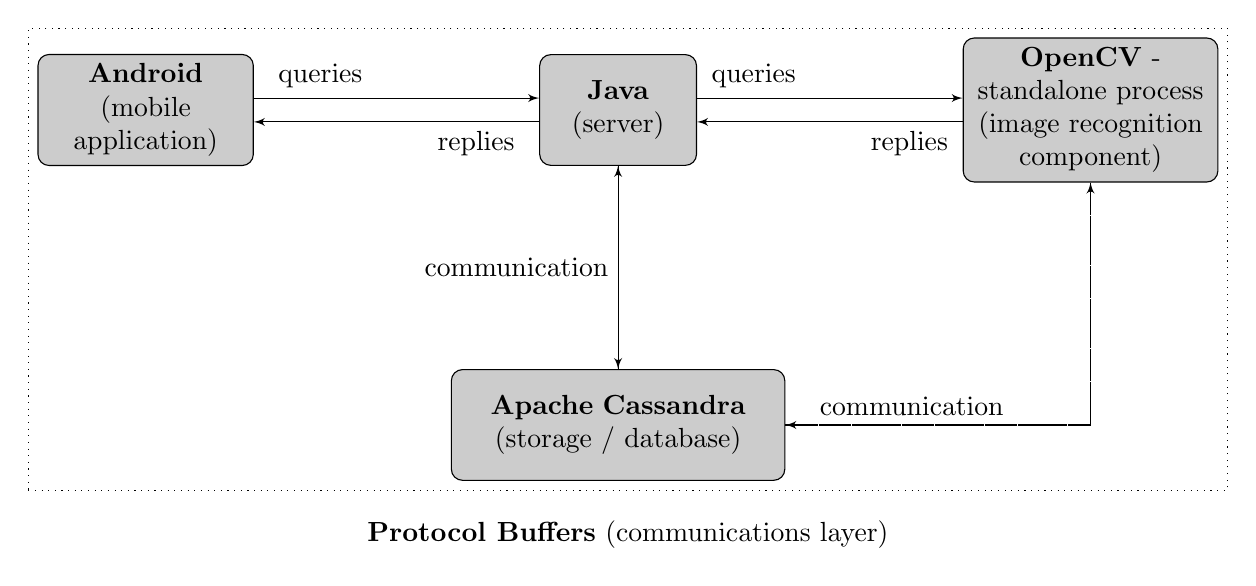
\begin{tikzpicture}[node distance = 2cm, auto]
    % Place nodes
    \node [block, text width=2.5cm] (app) {\textbf{Android} (mobile application)};
    \node [block, right of=app, node distance=6cm] (server) {\textbf{Java} (server)};
    \node [block, below of=server, node distance=4cm, text width=4cm] (db) {\textbf{Apache Cassandra} (storage / database)};
    \node [block, right of=server, node distance=6cm, text width=3cm] (ai) {\textbf{OpenCV} - standalone process (image recognition component)};
    % Draw edges
    \path [line] ([yshift=1ex] app.east) -- node [above, text width=3cm, align=left] {queries} ([yshift=1ex] server.west);
    \path [line] ([yshift=-1ex] server.west) -- node [below, text width=3cm, align=right] {replies} ([yshift=-1ex] app.east);
    \path [line] ([yshift=1ex] server.east) -- node [above, text width=3cm, align=left] {queries} ([yshift=1ex] ai.west);
    \path [line] ([yshift=-1ex] ai.west) -- node [below, text width=3cm, align=right] {replies} ([yshift=-1ex] server.east);    
    \path [line] (server.south) -- node [left, text width=4cm, align=right] {communication} (db.north);
    \path [line] (db.north) -- (server.south);  
    \path [line, dashed] (ai) |- (db);
    \path [line, dashed] (db) -| node [above, text width=3cm, near start] {communication} (ai);
	% Frame
	%\draw[thick,dotted] ($(app.north west)+(-0.25,0.75)$) rectangle ($(db.south east)+(5.75,-1)$);
	\node[draw=black, dotted, fit=(app) (ai) (db), ] (comm) {};
	\node[below of=comm, node distance=3.5cm] {\textbf{Protocol Buffers} (communications layer)};
\end{tikzpicture}
\end{center}
\caption{Technologies used in the system implementation}
\end{figure}
The main reasons for choosing these technologies are:
\begin{itemize}
\item \textbf{Java\tm} (server) $\rightarrow$ advanced network I/O and multithreading;
\item \textbf{Android}\footnote{http://developer.android.com/} (mobile application) $\rightarrow$ open-source, well documented, written in Java\tm;
\item \textbf{OpenCV}\footnote{http://opencv.willowgarage.com/} (image recognition component) $\rightarrow$ complex, efficient, versatile;
\item \textbf{Apache Cassandra}\footnote{http://cassandra.apache.org/} (storage) $\rightarrow$ excellent distributed performance, fast writes, caching;
\item \textbf{Protocol Buffers}\footnote{https://developers.google.com/protocol-buffers/} (communications layer) $\rightarrow$ high compression, works well with binary data.
\end{itemize}
\section{Communication}
For the \emph{Communication Layer}, we decided to use \emph{Google Protocol Buffers}. \emph{Protocol Buffers} are an extensible and efficient way to encode structured data, used by Google for most of their internal RPC protocols. This library has several advantages over the more widely used \emph{XML} or \emph{JSON}:
\begin{itemize}
	\item it is less verbose; setting values to keys is similar to \emph{XML} or \emph{JSON}, but the keys are not encapsulated in the final message;
	\item it is typed; this allows for data to be optimally encapsulated (\emph{e.g. 32-bit integer types will only take 4 bytes to encode});
	\item it works well with binary data (we will be using it to transfer images); on the other hand, \emph{XML} and \emph{JSON} work better when trying to encode markup text;
	\item it has built-in validation.
\end{itemize}
Also, given our current setup, we can easily avoid their disadvantages:
\begin{itemize}
	\item \emph{Protocol buffers} offer support only for C++, Java\tm\ and Python;
	\item a human-readable form can be obtained by parsing the message (\emph{e.g. in Java\tm, calling the \emph{toString()} method, or in C++, calling the \emph{DebugString()} method}).
\end{itemize}
Below is an extract from an example message used by our application:
\begin{lstlisting}
	// Next id = 5
	message DetectedObject {
		enum DetectedObjectType {
			UNKNOWN = 1;
			BUILDING = 2;
		}
		optional DetectedObjectType object_type = 1;
		optional ObjectMetadata metadata = 2;
		required string id = 3;
		optional bytes cropped_image = 4;
	}
\end{lstlisting}
The definitions for the \emph{Communication layer} messages are stored in the \textbf{/proto} directory. They are compiled using the \textbf{protoc} compiler. Below is an extract from the \emph{Protocol Buffers} \emph{Makefile}:
\begin{lstlisting}
	java:
		protoc --java_out=. comm.proto image_features.proto
		cp -r com/ ../AndroARComm/src/
\end{lstlisting}
Issuing the command \emph{make java} will result in the creation of \emph{Java classes}, stored in corresponding \emph{.java} files.
All the objects representing messages will be \emph{immutable} and will be created with the help of a dedicated \emph{Builder}. Below are some examples of methods created for the \emph{DetectedObject} class:
\begin{lstlisting}
	// builder
	public DetectedObject.Builder newBuilder();
	// getters
	public boolean hasObjectType();
	public boolean hasCroppedImage();
	public DetectedObjectType getObjectType();
	public String getId();
	public ByteString getCroppedImage();
	// serialization and communication
	public byte[] toByteArray();
	public static DetectedObject parseFrom(byte[]);
	public void writeTo(OutputStream output);
	public static DetectedObject parseFrom(InputStream input);
\end{lstlisting}
The \emph{DetectedObject.Builder} class has all the above methods, plus their corresponding \emph{setters} and a few more \emph{serialization and communication} methods:
\begin{lstlisting}
	// setters
	public DetectedObject.Builder setObjectType(DetectedObjectType value);
	public DetectedObject.Builder setId(String id);
	public DetectedObject.Builder setCroppedImage(ByteString value);
	// serialization and communication
	public DetectedObject.Builder mergeFrom(Message other);
	\end{lstlisting}
Creating the \emph{simplest}, but still \emph{valid}, DetectedObject message can be done as follows:
	\begin{lstlisting}
	DetectedObject detected_object =
	DetectedObject.newBuilder().setId("hello world").build();
\end{lstlisting}

\section{Server}
The server must be able to deal with the following aspects:
\begin{enumerate}
	\item be easy to distribute;
	\item allow multiple, simultaneous remote connections;
	\item easily implement an interface with the database;
	\item implement or interface with the image recognition component;
\end{enumerate}
The first three aspects are easier to implement using Java\tm, by making use of its more advanced \emph{network I/O} and \emph{multithreading} capabilities.

We decided to decouple the fourth aspect in a separate component, implemented in C++. We had the following aspects in mind:
\begin{itemize}
	\item optimization of CPU-bound components;
	\item most image recognition libraries and frameworks offer C/C++ support.
\end{itemize}
The server's main attributions are to \emph{ensure communication} and to \emph{correctly modify and forward messages} between all components.

The entire \emph{communication layer} is implemented by the server uses \textbf{TCP}. We are using reliable connections to be able to parse the messages we receive (binary encoded) and to ensure consistency of data throughout the system.

When a new client attempts to connect to one of the server instances, a new object is chosen from a \emph{threadpool} of \textbf{Client Connections}. Also, a new object is chosen from a \emph{pool} of \textbf{Database Connections}. Instead of the \emph{Client Connection object} creating its own \emph{database connection}, we have opted to use a pool of \emph{database connection} clients to allow for more instances to be used with each server, mainly to reduce the overhead of creating connections when issuing \emph{small and short-lived queries}.

For our current prototype, we have chosen to implement a \emph{many-to-one} communications model between the \emph{server} (more specifically the \emph{client connections}) and the \emph{image recognition component}. This has to do mainly with threading and synchronization being tedious to implement in C++. However, communication in the Java\tm\ server-side has been implemented with consideration to a future transition to a \emph{many-to-many} communications model. We are currently using a \emph{thread-safe queue} in order to serialize requests sent to the \emph{image recognition component}.

\subsection{Caching}
We implemented a caching system to take advantage of the fact that database queries for objects in a user's line of sight change very little over time, due to slow movement speed.

However, in order to use the caching system to its full potential, we must ignore the user's orientation when querying the database. Our implementation for the caching system queries the database for all the objects surrounding the user. It then stores them in the cache, but only serves the objects that are located in the user's line of sight (\emph{Figure} \ref{fig:caching}, \emph{left}). When another query is issued from the mobile application, the caching system only needs to query the database for objects in the unknown area (\emph{Figure} \ref{fig:caching}, \emph{right}).

\begin{figure}[H]
\begin{center}
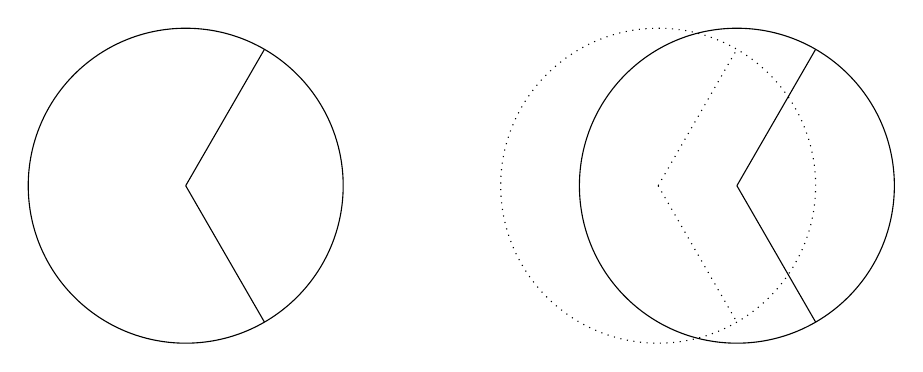
\begin{tikzpicture}
	\draw (0, 0) circle (2cm);
	\draw (0, 0) -- +(-60:2cm);
	\draw (0, 0) -- +(60:2cm);
	\draw [dotted] (6, 0) circle (2cm);
	\draw [dotted] (6, 0) -- +(-60:2cm);
	\draw [dotted] (6, 0) -- +(60:2cm);
	\draw (7, 0) circle (2cm);
	\draw (7, 0) -- +(-60:2cm);
	\draw (7, 0) -- +(60:2cm);
\end{tikzpicture}
\end{center}
\caption{Example of how the caching system works}
\label{fig:caching}
\end{figure}

\section{Storage}
	\subsection{CAP Theorem}
	\newtheorem{capthm}{Theorem}
	\begin{capthm}
	It is impossible for a distributed computer system to provide all of the following three guarantees:
	\begin{itemize}
		\item Consistency
		\item Availability
		\item Partition-tolerance
	\end{itemize}
	\end{capthm}
	This theorem was proposed as a conjecture by Eric Brewer at the 2000 Symposium on Principles of Distributed Computing (PODC). The formal proof was published in 2002\cite{cap}.
	
	\subsection{Database options}
	There are two directions of design and implementation for databases:
	\begin{enumerate}
		\item \textbf{ACID}, which stands for \emph{atomicity, consistency, isolation and durability}. Databases that implement \emph{ACID} include \emph{MySQL, SQLite};
		\item \textbf{BASE}, which stands for \emph{basically available, soft state, eventually consistent}. Databases that implement \emph{BASE} include \emph{Apache Cassandra, MongoDB}.
	\end{enumerate}
	There is also another classification of database types, based on the model they adhere to. The two most common classes of databases are:
	\begin{enumerate}
		\item \textbf{RDBMS} (stands for \emph{relational database management system}). Databases adhering to this model will have ACID properties and will typically use SQL (structured query language);
		\item \textbf{NoSQL}. NoSQL databases do not adhere to the RDBMS model. They typically do not use SQL as their query language and don't offer ACID properties. Most of these databases focus on the \emph{availability} and \emph{partition-tolerance} aspects stated in the CAP theorem, providing \emph{eventual consistency} within a \emph{distributed, fault-tolerant architecture}.
	\end{enumerate}
	
	Most database implementations fall into only one of the two classes. However, we must note that some implementations are \emph{hybrid}, such as the latest version of \textbf{PostgreSQL}.
	
	When choosing the database model, we must keep in mind several aspects:
	\begin{enumerate}
		\item \textbf{What the queries that we must reply to are}. The possible database queries are:
		\begin{enumerate}
			\item \emph{Return all the objects in the line of sight given a GPS position and an orientation}.
			\item \emph{Return images and features for an object, optionally sorted by rank}.
			\item \emph{Return metadata for an object (or a list of objects)}.
			\item \emph{Store an image and the detected objects that appear in it}.
		\end{enumerate}
		\item \textbf{What is the rate of occurrence of these queries}. Most of the queries that will be sent to the databases are
		\begin{enumerate}
			\item \emph{Return all the objects in the line of sight given a GPS position and an orientation}.
			\item \emph{Return (the best) images and features for an object}.
			\item \emph{Return metadata for an object (or a list of objects)}.
		\end{enumerate}
		with the most common being a combination between the first 2: \emph{Return (the best) images and features} --- \emph{for all the objects in the line of sight given a GPS position and an orientation}.
		\item \textbf{Consistency}. Before we decide whether we always need consistency or we can manage with eventual consistency, we must observe how the database can change over time.
		
		The database \textbf{replies} might change if one of the following events occur:
		\begin{enumerate}
			\item a store request appears and a new image is stored in the database;
			\item after a query, the ranking for the instances of objects changed (\emph{i.e. an instance of an object becomes more or less successful}).
		\end{enumerate}
		Given these possible situations, we can manage with \emph{eventual consistency}, because:
		\begin{itemize}
			\item a new instance of an object will not greatly affect the performance of the system, since determining whether an object appears in an image or not is done using more than one instances;
			\item ordering of object instances based on their success will not be drastically changed, since we can safely assume that the \emph{best} instances tend to remain at the top and the \emph{worst} instances tend to remain at the bottom.
		\end{itemize}
		\item \textbf{Latency}. The most common type of query needs to be answered as fast as possible, in order to reduce round-trip time. A distributed database is preferrable because we can easily ensure load balance.
	\end{enumerate}
	Due to all the aspects stated above, we decided to use a \emph{NoSQL} database. There are many \emph{NoSQL} database implementations, some of which being presented below, along with their features:
	\begin{center}
			\begin{tabularx}{\linewidth}{|l|X|}
				\hline
				\textbf{MongoDB}\footnote{http://www.mongodb.org/} & best used for dynamic queries over data that changes little over time\\
				\hline
				\textbf{Cassandra}\footnote{http://cassandra.apache.org/} & BigTable-like, highly-distributed, fast-write database\\
				\hline
				\textbf{HBase}\footnote{http://hbase.apache.org/} & best used in conjunction with Hadoop and HDFS\\
				\hline
				\textbf{Redis}\footnote{http://redis.io/} & best used for data that changes rapidly (\emph{i.e. communication}), but is limited in size\\
				\hline
				\textbf{Riak}\footnote{http://wiki.basho.com/} & the \emph{light} version of \emph{Cassandra}, with a trade-off in scalability\\
				\hline
				\textbf{VoltDB}\footnote{http://voltdb.com/} & a scalable, consistent and highly available multi-master database\\
				\hline
			\end{tabularx}
		\end{center}
	Given the use-case and restrictions of our application:
	\begin{itemize}
		\item Java\tm\ API,
		\item scalability,
		\item fast queries,
	\end{itemize}
	the top selections were \emph{MongoDB} and \emph{Apache Cassandra}. We will compare the two in the following section.
	\subsection{MongoDB vs. Apache Cassandra}
	\subsubsection*{API; Supported Languages}
	\textbf{MongoDB} is the best supported database from all those presented above. It has support for most of the programming languages and offers an API that retains some features from SQL.
	\noindent\textbf{Cassandra} offers a Java\tm\ API using \emph{Thrift}, a custom binary protocol. Database operations are rather tedious, but wrappers exist that easen up most of the operations (\emph{i.e. Hector}\footnote{http://hector-client.github.com/hector/}).
	\subsubsection*{Scalability}
	\textbf{MongoDB} is easy to set-up if only a single server is used.
	
	\noindent\textbf{Cassandra}, however, has the advantage of being more reliable when using more server instances. It has a no-single-point-of-failure architecture and more options for better management of data (\emph{i.e. replication factor, replication strategy, read/write quorum}). Also, Cassandra is easier to set-up in a multi-server environment, since all nodes are homogenous.
	\subsubsection*{Fast Queries}
	
	\indent\textbf{MongoDB} has more advanced support and flexibility for indexes. However, the main disadvantage of MongoDB is that it has a \textbf{global write-lock}, making large amounts of writes more problematic.
	
	\noindent\textbf{Cassandra}'s architecture performs extremely well when many \emph{writes} occur, offering constant-time writes, no matter how large the current database is.
	
	\subsection{Database Choice}	
	After comparing the top two choices for the database, we decided to use \textbf{Apache Cassandra} \cite{cass} as the database for our application.
	
	\subsection{Database Schema}
	Given that we are using a \emph{NoSQL} database, before we explain the \emph{database schema}, we need to offer definitions to the terms we will use:
	\begin{center}
	\begin{tabularx}{\linewidth}{lcX}
		\textbf{column} & $\rightarrow$ & a tuple of \emph{key}, \emph{value} and \emph{timestamp}; imagine this as a cell inside a SQL table;\\
		\textbf{supercolumn} & $\rightarrow$ & a group of \textbf{columns} with the same \emph{key}; imagine this as a tuple of \emph{key}, \emph{value} and \emph{timestamp}, where the \emph{value} field is a collection of columns (\emph{i.e. a map});\\
		\textbf{column family} & $\rightarrow$ & a collection of \textbf{columns}; imagine this as a SQL table;\\
		\textbf{keyspace} & $\rightarrow$ & a collection of \textbf{column families} and \textbf{supercolumn families}; imagine this as a SQL database.\\
	\end{tabularx}
	\end{center}
	We can now illustrate the \emph{database schema}. Our project's \emph{keyspace} will contain :
	\begin{itemize}
		\item \emph{1 column family} to store images and their features;
		\item \emph{1 supercolumn family} to store objects associated to images.
	\end{itemize}

	\begin{figure}[H]
	\begin{center}
		\begin{tabularx}{\linewidth}{|l|X|}
				\hline
				\multicolumn{2}{|c|}{\textbf{Image features}} \\
				\hline
				key & row key. This is the image's hash (string) \\
				\hline
				image-contents & the binary representation of the image (bytes) \\
				localization & the binary representation of the localization features \emph{Protocol Buffers} message, containing GPS position and compass orientation (bytes) \\
				\textbf{gps-latitude} & the GPS latitude where the image was taken (float) (\textbf{index}) \\
				\textbf{gps-longitude} & the GPS longitude where the image was taken (float) (\textbf{index}) \\
				num-objects & number of detected objects that appear in this image \\
				objectX & the id of detected object X (string) \\
				croppedX & the cropped image of detected object X (bytes)\\
				cvX & the features for the cropped image of detected object X. This is the binary representation of a \emph{Protocol Buffers} message that encapsulates all computed features (bytes) \\
				\hline
			\end{tabularx}
	\end{center}
	\caption{Image features column family}
	\end{figure}	
	
	\begin{figure}[H]
	\begin{center}
		\begin{tabularx}{\linewidth}{|l|l|X|}
				\hline
				\multicolumn{3}{|c|}{\textbf{Object instances}} \\
				\hline
				key & \multicolumn{2}{X|}{row key. This is the object's ID (string)} \\
				\hline
				metadata & object-name & name of the object (string) \\
				& object-description & a short description of the object (string) \\
				\hline
				image-index & first-available-image-id & the first available image id (integer) \\
				\hline
				imageX & image-hash & the hash of the cropped image containing the current object (string) \\
				& image-contents & the contents of the large image containing the current object (bytes) \\
				& cropped-image-contents & the contents of the cropped image representing the current object (bytes) \\
				& \emph{distance-to-viewer} & the distance between the viewer and the object (float) (\emph{optional}) \\
				& \emph{inferred-gps-position} & the inferred GPS position of the object -- a binary representation of the \emph{Protocol Buffers} localization features message (bytes) (\emph{optional}) \\
				\hline
			\end{tabularx}
	\end{center}
	\caption{Object instances column family}
	\end{figure}
For the implementation of the database queries, we decided to use \emph{Hector}, a high-level Java client for \emph{Apache Cassandra}. Its main advantages are:
\begin{itemize}
	\item object oriented interface;
	\item type-safety;
	\item encapsulation of the \emph{Thrift} API.
\end{itemize}
	
\section{Image Recognition Component}
\subsection{Why a Separate Server}
As stated above, we decided to implement the image recognition component as a separate server, written in C++. This is mainly because:
\begin{itemize}
	\item the image recognition component is CPU intensive. It is easier and more cost-effective to differentiate between \emph{I/O intensive} and \emph{CPU intensive} components. For example, Amazon EC2 offers highly specialized instances for such types of applications.
	\item we are using the OpenCV library for image recognition, written in C++.
\end{itemize}
The \emph{image recognition component} contains implementations of:
\begin{enumerate}
	\item classes that implement the \emph{communication layer} between the \emph{server} and the \emph{image recognition component}, using the \textbf{TCP} stack;
	\item classes that extract and match features, giving a \emph{score} (or \emph{a level of confidence}) to the pair (\emph{query image, object instance});
	\item classes that remove incorrect matches.
\end{enumerate}
\subsection{The OpenCV Library}
OpenCV\cite{opencv} is a library of programming functions for computer vision software. Supported functions range from \emph{general image processing functions} and \emph{transformations} to \emph{feature extraction} and \emph{machine learning}.

OpenCV also provides a version for Android, which offers similar features. This will ease the process of splitting the computational work between the mobile application and the server.

The process of detecting whether an object appears in an image or not is done by extracting the features from the image and matching them against available object instances.

\subsection{Feature detection}
For feature extraction we experimented with two feature detectors:
\begin{enumerate}
	\item SIFT (\emph{Scale-Invariant Feature Transform}) detector;
	\item SURF (\emph{Speeded-Up Robust Feature}) detector;
\end{enumerate}

\subsubsection{The SIFT Detector}
This detector was designed to be \textbf{invariant} to \emph{uniform scaling} and \emph{changes of orientation} and \textbf{partially invariant} to \emph{changes in illumination} and \emph{affine transformations}.

The \emph{SIFT} detector uses several techniques, algorithms and heuristics to extract features (\cite{sift1},\cite{sift2},\cite{sift3}). These can be divided into the following steps\footnote{http://www.aishack.in/2010/05/sift-scale-invariant-feature-transform/}:
\begin{enumerate}
	\item \textbf{generate scale spaces}. \emph{SIFT} expands on the idea of correctly removing unnecessary details by using \emph{gaussian blur}. It computes \emph{scaled-down} sets of \emph{increasingly blurred} images, called \emph{octaves};
	\item \textbf{compute the LoG - Laplacian of Gaussians}. This is achieved using an approximation of the laplacians (\emph{i.e. second derivative}), using \emph{DoG - Difference of Gaussians};
	\item \textbf{find keypoints}. This is done by computing local maxima and local minima on the previously computed \emph{DoG} images;
	\item \textbf{remove uninteresting keypoints}. Most of these are located on edges, or are in low-contrast areas;
	\item \textbf{associate orientation information with keypoints}. This is done by computing a \emph{histogram} for the \emph{magnitude} and \emph{orientation} values. The orientation will be chosen according to the highest values in the histogram (we should note that, in this step, a single keypoint can be duplicated, should more than one histogram maxima exist);
	\item \textbf{compute features}. A window of $16\times16$ pixels is chosen, with the keypoint in the center. This is then divided into $16$\ $4\times4$ windows; gradient magnitudes and orientations are computed for each pixel in each window and placed into an 8-bucket histogram, scaled according to the magnitude (each bucket corresponds to a $45^\circ$ arc). 128 values will result ($16$ windows $\times 8$ buckets) which, after normalization, form the \emph{feature vector}.
\end{enumerate}

\subsubsection{The SURF Detector}
This detector was designed as an improvement to the \emph{SIFT} detector. It is claimed to perform reasonably well in terms of quality, compared to the \emph{SIFT} detector, while also being several times faster \cite{surf}. Much of this performance increase is due to:
\begin{itemize}
	\item using local intensity differences around keypoints, \emph{i.e. they apply the following two kernels}:
	\begin{figure}[H]
		\begin{center}
			\begin{tabular}{|c|c|c|c|}
				\cline{1-2}\cline{4-4}
				-1 & 1 & & -1 \\
				\cline{1-2}\cline{4-4}
				\multicolumn{3}{c|}{ } & 1 \\
				 \cline{4-4}
			\end{tabular}
		\end{center}
	\end{figure}
	\item in an intermediary step, computing the \emph{Integral Image}, that will allow constant computation of the sum of intensities (\emph{i.e. area}) of any rectangular section.
\end{itemize}

\subsection{Feature Matching}

We experimented with a \emph{brute-force, k-nearest-neighbor} algorithm to select features, as well as with the \emph{FLANN-based} matcher. We found that, although the \emph{FLANN-based} matcher is randomized, it achieves similar results in terms of quality, and is roughly 3 times faster than the \emph{brute-force} matcher.
\begin{figure}[H]
	\begin{center}
		\begin{tabular}{|c|c|c|}
			\hline
			\textbf{Number of images in test} & \textbf{Brute-force matcher} & \textbf{FLANN-based matcher}\\
			\hline
			8 images & 10 seconds & 3 seconds\\
			12 images & 14 seconds & 4 seconds\\
			\hline
		\end{tabular}
	\end{center}
	\caption{Comparison of run-time for a test suite}
\end{figure}
This is because the \emph{FLANN} matcher uses more optimized data structures, which allow for faster \emph{k-nearest-neighbor} algorithms to be implemented:
\begin{itemize}
	\item \emph{K-D trees} and \emph{Randomized K-D trees};
	\item \emph{K-means trees}.
\end{itemize}

\subsection{Optimization}
The use-case of our application makes it difficult for feature detectors and matchers to achieve good performance:
\begin{itemize}
	\item the target objects we are matching against are buildings. While there are several landmarks and buildings that have distinct features (\emph{i.e. The Eiffel Tower, The Guggenheim Museum}), most of them are similar, especially if they are removed from their context (\emph{i.e. GPS position, background}). For example, consider all the apartment buildings in Eastern Europe, or the similarities between \emph{L'Arc de Triomphe} in Paris and the one in Bucharest,
\end{itemize}
or good latency:
\begin{itemize}
	\item feature matchers work in nearly \emph{$O(nlogn)$ time}, with some (i.e. \emph{FLANN}) managing to work in $.1$ of that. This means that it is impossible to try and find each and every possible object in an image (\emph{e.g. if we had $10000$ tagged objects and $10$ instances for each of them, we would have to run the matching algorithm against $100000$ pairs}).
\end{itemize}
We therefore need to improve both the accuracy and the latency of the matching process.

\subsubsection{Finding correct subsets of images}
As discussed above, we implemented a heuristic to detect which objects can be present in a query image. This takes into account the \emph{GPS position} and the \emph{compass orientation} of the user.
In addition to that, we implemented a system for ranking instances of objects. For the objects that are in the user's line of sight, we will choose the top $X$ instances, based on this ranking system.
The ranking system will work as follows:
\begin{itemize}
	\item when the rate of valid matches between the query image and a particular instance of an object is higher than some threshold $T$, then the image receives a boost $B_+$;
	\item when the rate of valid matches between the query image and a particular instance of an object is lower than that threshold, then the image receives a penalty of $B_-$.
\end{itemize}
The ratio $B_+ : B_-$ should be approximately $10 : 1$. We must take into account the fact that we will have instances representing different sides (angles) of the object; therefore, matching between a query image representing an angle of the building and a valid instance representing a completely different angle should not incur a significant penalty. Conversely, the bonus should be significant enough to boost a valid instance even if it received penalties for images from different angles.

\subsubsection{Removing uninteresting matches}
We implemented a system which allows purging features and matches that aren't relevant. For example, buildings' corners might perform extremely well (\emph{i.e. corners from the query image and an object instance might be matched with extremely low distance --- or high confidence}), but that might not relevant for the matching process. Another example are features that have very high distance --- or low confidence when matched (\emph{i.e. an advertising panel that appears in both the query image and the object instance, but shows different ads}).

We were interested in implementing and experimenting with several ideas of \emph{purging} uninteresting features and matches, therefore we are using a generic approach by using the \emph{abstract} \textbf{MatchPurger} \emph{class} to allow for easy injection of more algorithms and heuristics.

\subsubsection{Clustering of features}
One of the most basic ways of removing invalid feature matches is clustering. We are computing the \emph{mean} distance of matches, as well as the \emph{standard deviation}:
$$
mean = \frac{\sum_{m \in Matches}distance(m)}{|Matches|}
$$
$$
std = \sqrt{\frac{\sum_{m \in Matches} (distance(m) - mean)^2}{|Matches|}}
$$
and then removing the matches outside the range:
$$
(mean - threshold * std, mean + threshold * std)
$$

\subsubsection{Removing low-performance features}
Even if we associate objects not only with the images they appear in, but also with their geographic context, problems still remain with similar architecture. With the same example in mind, of the architecture of buildings in Eastern Europe, we can observe two main issues that might result in incorrect matching:
\begin{enumerate}
	\item adjacent buildings with similar features in the query image;
	\item repetitive sections in the buildings (\emph{e.g. windows}).
\end{enumerate}
To cope with these problems, we have implemented a way to remove the matches that have the following property: \emph{the feature from the query image can be best matched with 2 or more features in the object's instance image, with roughly the same probability}. We are removing the matches from both the query image's point of view, and the object's instance point of view, as follows:
\begin{enumerate}
	\item compute all the possible matches between the \emph{query image} and an \emph{object's instance}. For each possible match, we will store at most 2 pairs $(F, f)$, where $F$ is the feature from the \emph{query image}, and $f$ is a possible matched feature in the \emph{object instance}. These represent the top 2 choices, based on the distance between $F$ and all possible $f$;
	\item we ignore all matches for which the top 2 pairs $(F, f)$ have a relative difference in distance lower than some threshold:
	$$
	\frac{\min(dist(F, f1), dist(F, f2))}{\max(dist(F, f1), dist(F, f2))} < 1 - \varepsilon
	$$
	This means that are throwing out matches for which the top choices are equally probable;
	\item we execute the steps above for the reversed pair of images (\emph{i.e. the object instance and the query image};
	\item we remove all matches from the first set, that do not have a corresponding match in the second set (\emph{i.e. all matches that were found for the pair \emph{(query image, object instance)}, but not for the pair \emph{(object instance, query image)})}
\end{enumerate}
In our tests, we achieved a rate of removal of $90\% - 96\%$ after the first 3 steps. The final step resulted in an additional removal of roughly $50\%$ of the remaining matches.

\subsubsection{Interpreting the geometric properties of matches}

Another aspect we must consider is the possible transformations on objects.
In most of the use cases (the typical, normal use-case), it is impossible for the following transformations to occur:
\begin{itemize}
	\item major skew;
	\item mirror;
\end{itemize}
very unlikely for:
\begin{itemize}
	\item rotation;
\end{itemize}
and very likely for:
\begin{itemize}
	\item minor skew due to the camera lens;
	\item translation;
	\item scale.
\end{itemize}

This will allow us to impose some geometric restrictions on the matches. If we were to place the two images next to each other and draw lines between the matching key points, then the lines corresponding to the best matches will be parrallel (if the object and its instance in the query image are the same size) or skewed (if one of them is larger).
We can use the simple clustering algorithm stated above for the slopes.

\subsubsection{Fundamental Matrix. Epipolar lines. RANSAC}
For further match purging, we can take advantage of a simple observation: \emph{if matching is correct, the query image and a particular object instance can be seen as made by two cameras \emph{looking} at the same object}. This means we can take advantage of algorithms based on \emph{stereo-vision}.

The \textbf{epipolar line} of a particular point \emph{X} in the first image is an imaginary line on which the same point \emph{X}, seen by the second camera, can lie on.
The \textbf{fundamental matrix} is the mathematical relation between how a point from the first image is mapped in the second image.

Therefore, assuming that we know what the fundamental matrix is for a pair of images, we can purge all invalid matches. However, OpenCV needs at least \textbf{7 valid matches} in order to compute the fundamental matrix. We will use the \textbf{RANSAC} (RANdom SAmpling Consensus) algorithm to compute an estimation of the fundamental matrix. The idea behind RANSAC is to randomly select as few matches as possible, compute the fundamental matrix and then select all the other valid matches. Should any of the randomly picked matches be invalid, the RANSAC algorithm will ouput very few valid matches.

\vspace{1cm}

After applying the \textbf{Repetitive Features Purger} and the \textbf{RANSAC Match Purger}, we obtained excellent results:

\begin{figure}[H]
\begin{center}
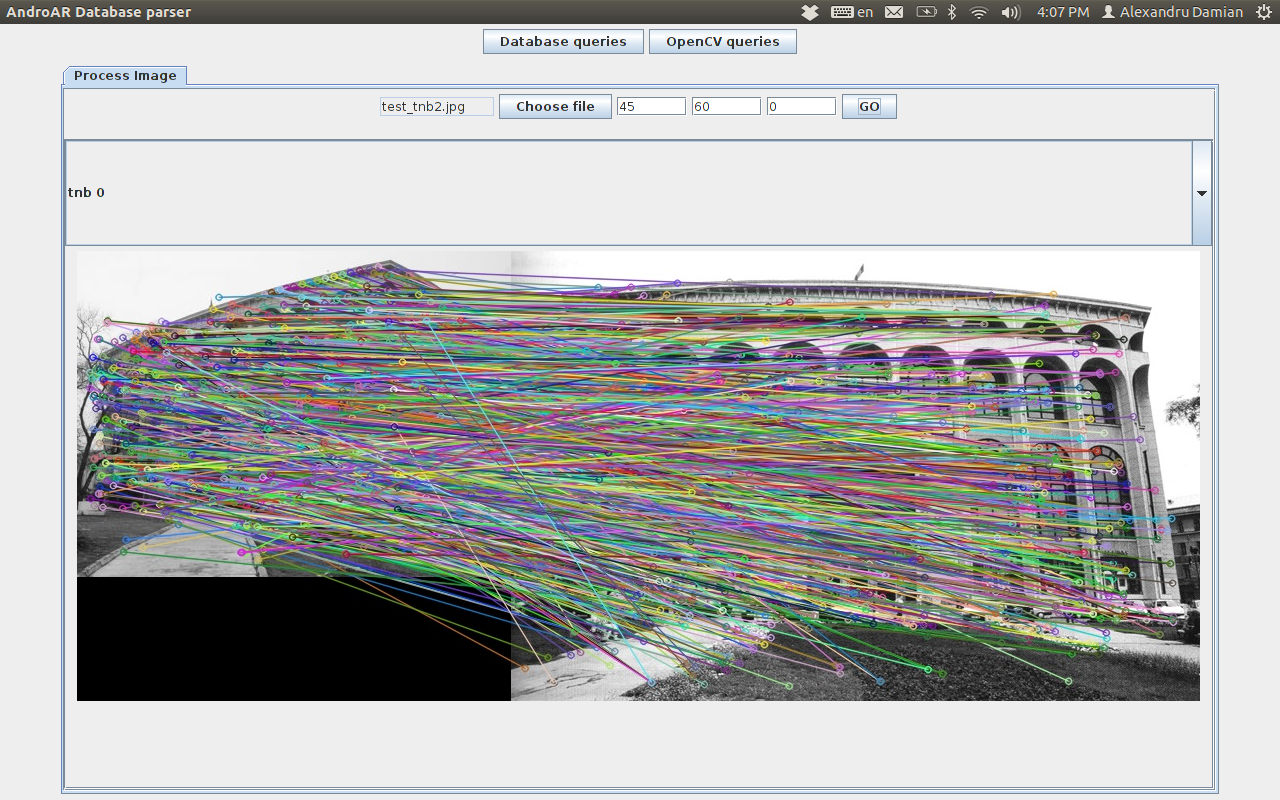
\includegraphics[width=7.9cm]{images/matches_before_purge.png}
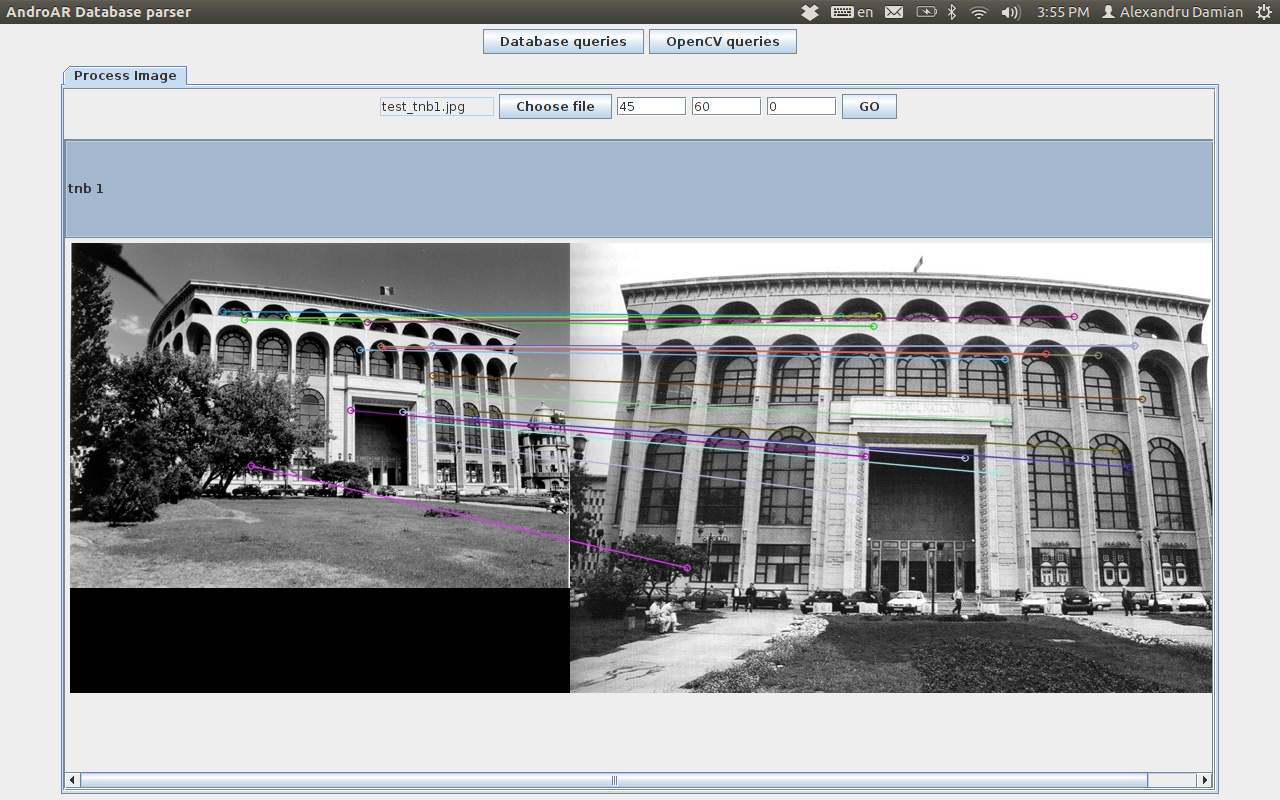
\includegraphics[width=7.9cm]{images/matches_after_purge.png}\\
left: before purging matches, right: after purging matches
\caption{Amount of invalid matches purged}
\end{center}
\end{figure}

\section{Testing GUI}
We needed a \emph{debug} version of the system that allowed visual inspection of the matching of features between the query image and all the instances of all the possible objects present in the user's line of sight.

We decided to implement the testing GUI using the Java\tm\ Swing API and use it as a standard desktop application. This way, we have several advantages:
\begin{itemize}
	\item we can control and fine-tune queries;
	\item by using a \emph{debug} version of the communication layer between the system's components, we can receive a reply containing significantly more information than the production version. This will allow us to compute image recognition performance statistics and to visually inspect the success of the matching algorithms we use.
\end{itemize}
and we remove the disadvantages of using a \emph{debug} mobile application:
\begin{itemize}
	\item visual inspection of the matching algorithms is tedious when using a mobile application, given fewer controls and smaller screen size;
	\item a mobile application will incur another step in the data's path from query to reply;
	\item we do not need the features we would normally use in the production version: real localization capabilities, real camera feed, etc.
\end{itemize}

\begin{figure}[H]
\begin{center}
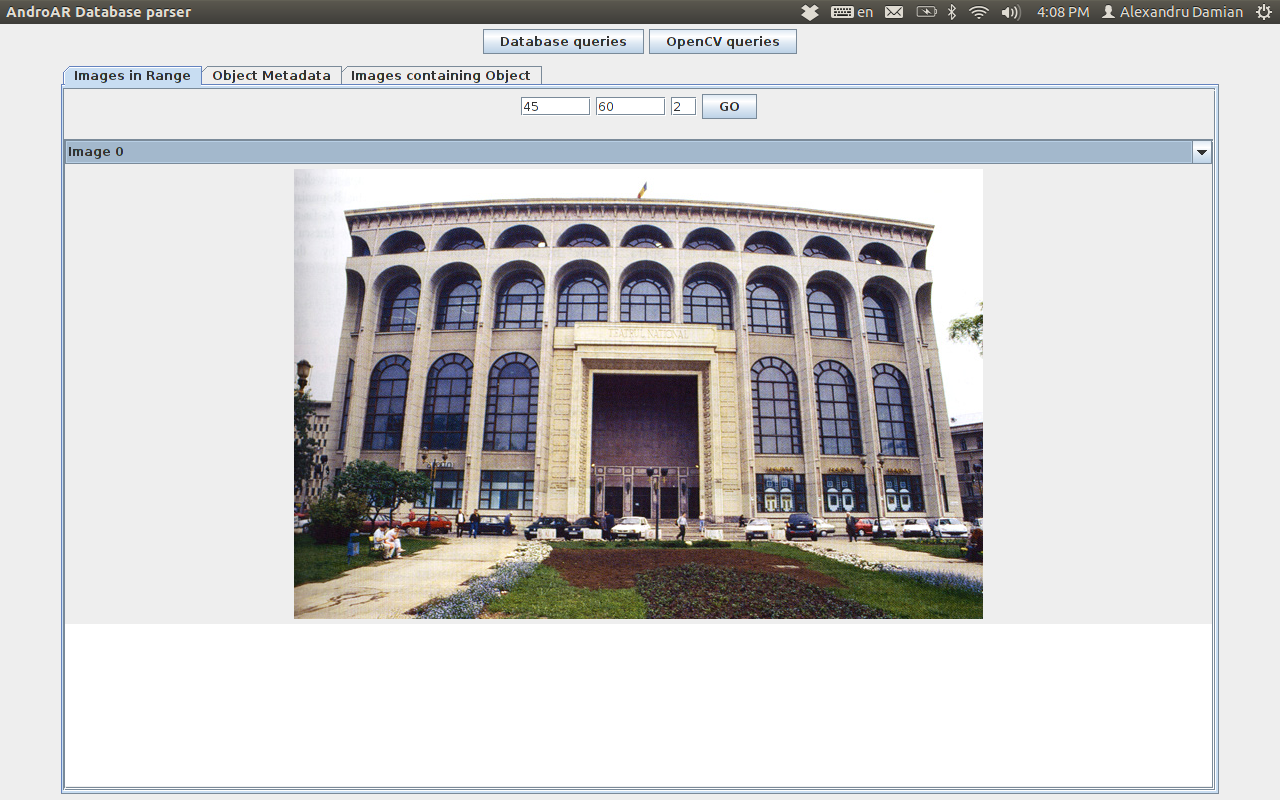
\includegraphics[width=8cm]{images/testing_gui_database_queries.png}
\caption{Database queries screen in the Testing GUI}
\end{center}
\end{figure}

\section{Mobile Application}
\subsection{Android Platform}
Mobile platforms are currently dominated by the \emph{Android} and \emph{iOS} platforms. We decided to use the \emph{Android} platform to implement the mobile application, mainly because:
\begin{itemize}
	\item the platform is open-source, well documented and supported by a large community;
	\item applications are written in Java\tm\ , which is consistent with our choice for the Communication library.
\end{itemize}
We implemented the mobile application to support the \emph{Gingerbread (2.3)} version of the \emph{Android} platform. More than 50\% of the \emph{Android} smartphones run the \emph{2.3} version, and 25\% more run newer versions. In addition to this, so far we do not need any of the new functionality of the newer versions. The mobile application is fully compatible with future versions, but not backwards.

The \textbf{interface} was created using XML layouts, as is recommended for Android to reduce load times.

\begin{figure}[H]
\begin{center}
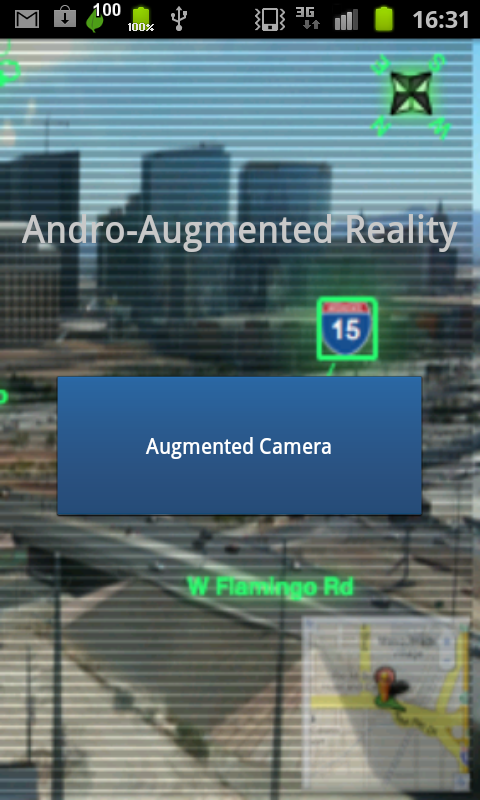
\includegraphics[width=8cm]{images/camera.jpg}
\caption{Main screen of the AndroAR prototype}
\end{center}
\end{figure}

\textbf{Camera integration} was implemented using SurfaceView\footnote{http://developer.android.com/reference/android/view/SurfaceView.html} and several callbacks issued when the camera view is initialized, changed or destroyed. Everytime the main camera preview (activity) is interrupted, the camera is stopped and a new camera instance is obtained when the activity is brought back to foreground.

\textbf{GPS positioning} and \textbf{compass orientation} were obtained using the android internals,
through listeners that update them when changed.

The \textbf{user experience} and \textbf{user interface} are clear and straightforward, allowing the user to receive replies from the servers on the camera preview main activity, but in the same time permitting screen captures to allow cropping and tagging of buildings. After the user has provided proper keywords and a description for the selected landmark, the information is sent to the server, using a TCP connection.
Image cropping was done using an android built-in intent and, thus, before and after actions were needed, in order to parse the newly obtained data. Also, as an improvement, saving an image to the storage space is done asynchronously, in background, by extending the AsyncTask\footnote{http://developer.android.com/reference/android/os/AsyncTask.html} class.

\begin{figure}[H]
\begin{center}
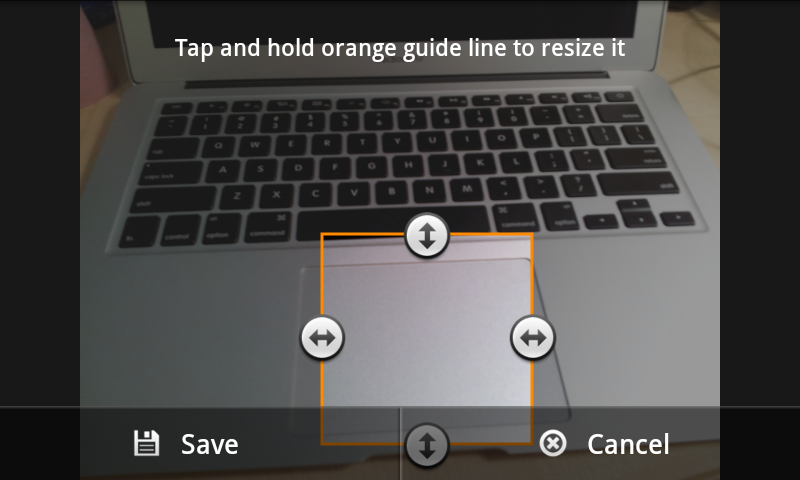
\includegraphics[width=8cm]{images/crop.png}
\caption{Screen caption of the image crop step in the AndroAR prototype}
\end{center}
\end{figure}

\begin{figure}[H]
\begin{center}
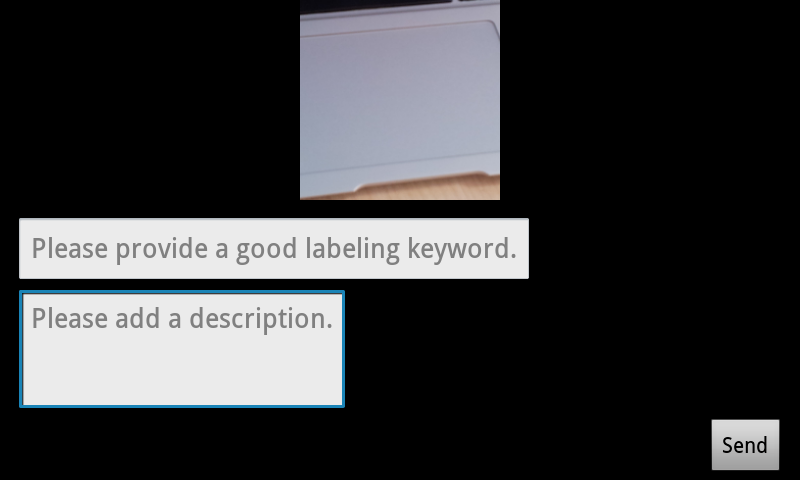
\includegraphics[width=7.9cm]{images/metadata.png}
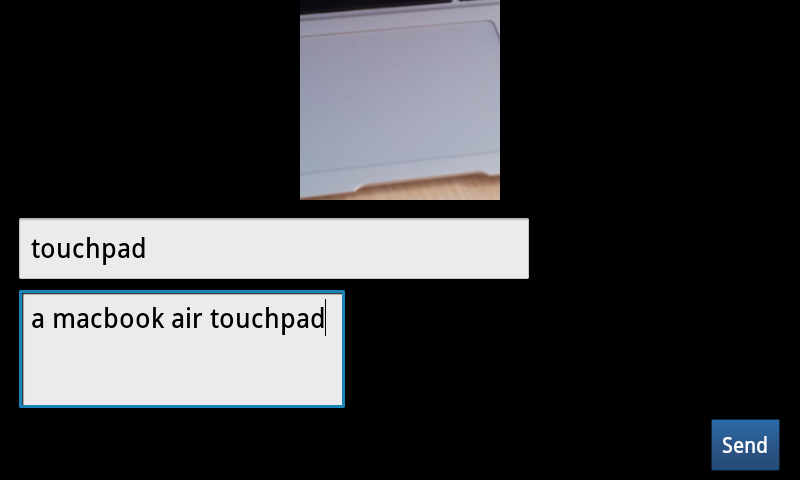
\includegraphics[width=7.9cm]{images/metadata_send.png}
\caption{Screen captions of the tagging step in the AndroAR prototype}
\end{center}
\end{figure}

\textbf{Note:} development of the Android application has been done by Andrei Petre\footnote{student at the Polytechnic University of Bucharest, Faculty of Automatic Control and Computers, second year}.

\section{Tools}
\label{sec:tools}
Apart from the techologies used in the implementation (\emph{Apache Cassandra, Protocol Buffers, OpenCV, Android}), we will present other tools used during development in the following list, along with some details:
\subsection*{Git. GitHub}
Git is currently one of the most feature-rich and easy-to-use version control systems. It has support for advanced features, such as branching and tagging. We used \emph{git} in conjunction with \emph{github.com}, a service that offers free hosting of open-source projects, using git. Features of \emph{github.com} include a visual interface to track changes in commited files, tickets and milestones.

\subsection*{Eclipse IDE\footnote{http://www.eclipse.org/}}
As one of the most popular IDEs on the market, Eclipse has numerous features:
\begin{itemize}
	\item code highlighting;
	\item auto-completion;
	\item refactoring tools (\emph{i.e. renaming of classes, functions and variables});
	\item auto-build;
	\item class-hierarchy navigation and search;
	\item plugins.
\end{itemize}

\subsection*{Ant\footnote{http://ant.apache.org/}}
Ant can be considered a replacement (or an enhancement) of the \emph{make} utility, designed specifically for Java\tm\ projects. It has the same functionality as \emph{make}, but uses XML and offers many shortcuts to ease the Java\tm\ build process.

\chapter{Results and Conclusions}
\label{chap:results}

We have successfully implemented and tested a prototype of the proposed application. 
\section{Installation}
Installation of the application is relatively straightforward, using Ant, but only assuming all prerequisites are met:
\begin{itemize}
	\item sun-java-1.6 (Java\tm\ compiler);
	\item libprotoc 2.4.* (Protocol Buffers compiler);
	\item opencv 2.3.* (OpenCV library);
	\item Cassandra 1.* (Cassandra database);
	\item Hector 1.* (Hector API, working on top of Cassandra).
\end{itemize}
For testing purposes, the following requirements are needed:
\begin{itemize}
	\item Android SDK, version 2.3 or higher;
	\item (\emph{optionally}) a smartphone running Android 2.3 or higher.
\end{itemize}
We successfully installed and ran end-to-end tests on:
\begin{itemize}
	\item \textbf{remote VPS}: quad-core Intel Xeon @ 3.2GHz, 2GB RAM;
	\item \textbf{localhost}: quad-core Intel I5M @ 2.4GHz, 4GB RAM.
\end{itemize}

Test results showed a reply latency of approximately $3$ seconds when a query using a 1920$\times$1080 resolution image was issued. Time spent on a query was divided as follows:
\begin{itemize}
	\item 40\% interaction between the server and database, along with forwarding queries;
	\item 40\% OpenCV processing;
	\item 20\% network time.
\end{itemize}
\section{Results}
We are extremely satisfied with the results we obtained in terms of latency and we target a 25\% to 50\% reduction when using smaller images and better caching.

In terms of performance, using the purgers presented in chapter \ref{chap:implementation} we have managed to achieve excellent results, even when matching \emph{difficult} buildings (\emph{i.e. buildings with common architecture or repetitive features}).

Latency tests were conducted using a verbose version of the mobile application, while performance tests were conducted using the Testing GUI, for visual inspection, backed by a suite of bulk tests ran against a separate, testing database.
\section{Problems}
During the development process, we encountered several problems:
\begin{itemize}
	\item \textbf{difficulty using Cassandra and Hector}. Cassandra is, by design, difficult to use programmatically, and the most efficient and easy-to-use solution is Hector. However, the API doesn't support all possible types of queries and is poorly documented. We were forced many times to reverse engineer test-cases in order to understand the correct usage and behaviour of Hector. 
	
	Also, debugging correct insertions in the database was tedious since a GUI to explore the database is not offered. Only a CLI client is available, which has its limitations, mainly because Cassandra is not typed (keys and values are stored as \emph{byte arrays}). We were forced to create unit tests for all types of queries (see \textbf{/AndroARServer/src/test/com/androar/CassandraDatabaseConnectionTest.java}).
	\item \textbf{matching}. The OpenCV library has many features and algorithms implemented to extract and match features. However, there is no out-of-the-box solution for our use-case. We had to research and implemenent heuristics, adapted to our use-case, in order to extract subsets of correct and relevant features and match those.
	\item \textbf{Protocol Buffers}. Protocol Buffers are extremely efficient and message definitions are intuitive and fast to write. However, setting up the environment needed to support them is rather tedious. Also, creating messages in Java\tm\ is more complex and more verbose than in C++.
	\item \textbf{communication between Java\tm\ and C++}. We had several issues with communication between the Java\tm\ and C++ components, mainly with data delivery through sockets.
	\item \textbf{debugging}. Creating and running tests to determine whether heuristics yield correct classifications was not difficult. However, we needed a more detailed view on the matching process, apart from the \emph{binary yes/no} results, a way to visually inspect the features that were matched. Thus, we implemented the testing GUI, along with a \emph{DEBUG}, \emph{more verbose} version of the communications layer.
	
	Below is an extract of some tests created for the matching process:
	\pagebreak
	\begin{verbatim}
	  ********** TEST 1 **********
	  image {
	    image_hash: "src/test/test_intercontinental.jpg"
	  }
	  detected_objects {
	    ...
	    id: "intercontinental"
	  }
	  ********** TEST 2 **********
	  image {
	    image_hash: "src/test/test_tnb1.jpg"
	  }
	  detected_objects {
	    ...
	    id: "tnb"
	  }
	  ********** TEST 3 **********
	  image {
	    image_hash: "src/test/test_tnb2.jpg"
	  }
	  detected_objects {
	    ...
	    id: "tnb"
	  }
	\end{verbatim}
	\item \textbf{Android}
		\begin{itemize}
			\item \textbf{communication}. When we implemented the query loop, we were faced with restrictions on the Android platform regarding blocking socket reads. 
			\item \textbf{camera}. All Android application are required to serialize access to the camera by using \emph{callbacks}. This poses several problems, because we have no control over when the callbacks will be executed and when camera frames will become available.
		\end{itemize}
\end{itemize}
\section{Conclusions}
During the development process of this system, we have gained deeper understanding of augmented reality research and image recognition algorithms. We have drawn the following conclusions:
\begin{enumerate}
	\item ambient intelligence and, in particular, augmented reality, have gained much momentum in the past years; research and development in these fields are offering more advanced hardware and software (\emph{i.e. Google Glasses, BMW head-up display}) and are moving towards integration of data from as many sensor types as possible;
	\item acquiring sensor data is not straightforward and is prone to errors; ambient intelligence applications must also deal with these errors;
	\item implementation of queries using the Cassandra database was tedious. Had we known that, we would have most likely chosen MongoDB to store our data.
	\item the system design was successfuly implemented and a prototype is available. It works as expected and offers high quality results. However, latency is still an issue and future work is needed to ensure a seamless experience for future users. 
	\item the direction we chose for the design of this system is also pursued by major companies and research institutions, which contributes to proving the validity of our idea.
\end{enumerate}

\chapter{Future Work}
\label{chap:conclusions}
Our plan is to make \emph{AndroAR} production ready. This will require both the implementation of new features and the optimization of existent ones.

\section*{Support for Sparse Queries}
As noted in the previous chapters, it is impossible to issue queries for every frame of the camera feed, whether our target is \emph{30 frames per second} (because of the amount of queries) or \emph{1 frame per second} (because, even then, the reply will arrive delayed and will, thus, be out-of-sync). We need to implement a way to track objects in the camera feed; alternatively, we can understand how the phone moves and then infer object movement.

Detecting how the user moves their phone seemed the easier to implement choice. Our initial thoughts were to use the internal \emph{accelerometer} to detect the direction and speed of the phone movement, since there are many smartphones with this hardware embedded. We would then have had to compute the distance covered and translate the bounding boxes accordingly. However, we found it too tedious and unsecure to compute distances based on the accelerations: if we are issuing queries every $4-5$ seconds, then we mostly rely on computing how the images translated to correctly display the bounding boxes; even the smallest error in the accelerometer sampling will result in a huge offset during these $4-5$ seconds \emph{(due to integrating acceleration \emph{twice} to obtain distance)}.

Therefore, we decided to detect translations using the \emph{OpenCV} library for Android to track features in images. This will allow for more accurate computation of translations.

\section*{Passive Example Generation}
Using the \emph{OpenCV} library for feature tracking will also allow us to generate more examples, by storing instances of objects in frames adjacent to the one that generated a valid match, or to the one that was selected by the user to tag a building with metadata. A similar approach, called \emph{Predator}\footnote{http://info.ee.surrey.ac.uk/Personal/Z.Kalal/tld.html}, was already implemented, and achieved excellent results.

\section*{Image Normalization}
Most image recognition algorithms have low tolerance to lighting changes. The \emph{OpenCV} library transforms images to grayscale and normalizes intensities before attempting to extract any features.

However, we can do more and, for example, estimate the amount of lighting based on the current time of day (a feature we have available on any smartphone).

\section*{Inferring GPS Position}
Currently, when a storage request is issued, we assume that all objects that appear in the camera frame are located at the GPS position provided by the phone (\emph{i.e. all objects are stacked on top the current user's position}). It would be nice to be able to estimate the GPS position of objects, based on the user's viewport and the camera's focal length.

\section*{Database Improvements}
The current system design is homogenous. All information is stored in a single database (we refer here to a collection of machines, acting as a distributed database), even though it is clear that any query will interact with only a fraction of the database (\emph{e.g. queries that originate in Romania will not interact with the part of the database storing information for buildings located in the US}).

Given these geographical issues, we can take advantage of sharding:
\begin{figure}[H]
\begin{center}
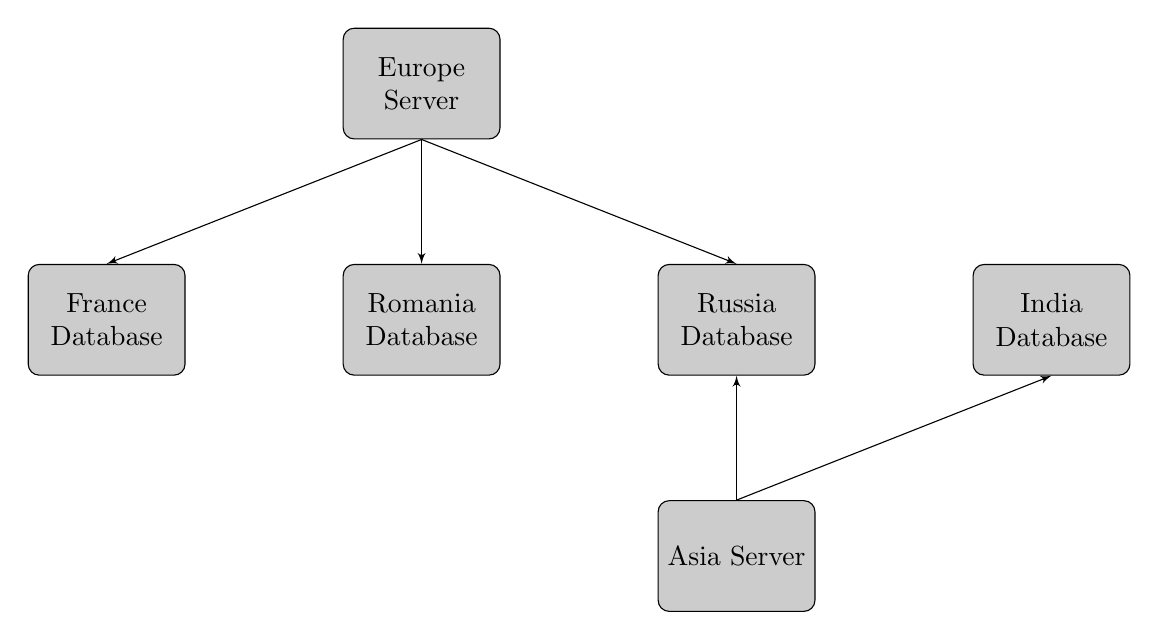
\begin{tikzpicture}[node distance = 2cm, auto]
    % Place nodes
    \node [block] (s_eu) {Europe Server};
    \node [block, below of=s_eu, node distance=3cm] (db_ro) {Romania Database};
    \node [block, left of=db_ro, node distance=4cm] (db_fr) {France Database};
    \node [block, right of=db_ro, node distance=4cm] (db_ru) {Russia Database};
    \node [block, right of=db_ru, node distance=4cm] (db_in) {India Database};
    \node [block, below of=db_ru, node distance=3cm] (s_asia) {Asia Server};
    % Draw edges
    \path [line] (s_eu.south) -- (db_fr.north);
    \path [line] (s_eu.south) -- (db_ro.north);
    \path [line] (s_eu.south) -- (db_ru.north);
    \path [line] (s_asia.north) -- (db_ru.south);
    \path [line] (s_asia.north) -- (db_in.south);
\end{tikzpicture}
\end{center}
\caption{Geographic explanation of the advantages of sharding.}
\end{figure}

\section*{Other Improvements}
At present, communication is done using \emph{Protocol Buffers}, over \emph{TCP}. We are planning to transition to \emph{UDP} or \emph{RTP}, protocols that are more suitable for media delivery. If so, \emph{Protocol Buffers} might become unsuitable and other solutions will have to be researched.

Also, security aspects will have to be considered. Some of the most common security precautions that will have to be implemented are:
\begin{itemize}
	\item prevention of \emph{denial of service} attacks;
	\item spam purging, when issuing store requests:
	\begin{itemize}
		\item if the building is already tagged in the database, we will treat the store request as a normal query to ensure validity and quality; we will store the instance only if the confidence of it representing the proposed building surpasses a certain threshold;
		\item if this is the first time the building is tagged, then we will rely on user validation. It would be nice to be able to search the web for the proposed building name and match the provided image against the top search results.
	\end{itemize}
	\item user accounts, most likely by using \emph{open authentification} (\emph{i.e. OAuth, Facebook login, Google login})
\end{itemize}

\pagebreak
\listoffigures

\begin{thebibliography}{99}
\bibitem{ist01}K. Ducatel, M. Bogdanowicz, F. Scapolo, J. Leijten, J-C. Burgelman, \emph{Scenarios for Ambient Intelligence in 2010}, 2001
\bibitem{aima}Stuart Russell, Peter Norvig, \emph{Artificial Intelligence: A Modern Approach}, Prentice Hall, Third Edition, 2010.
\bibitem{dud01}Richart O. Duda, Peter E. Hart, David G. Stork, \emph{Pattern Classification}, Wiley-Interscience, 2001.
\bibitem{cap} Nancy Lynch, Seth Gilbert, \emph{Brewer's conjecture and the feasibility of consistent, available, partition-tolerant web services}, ACM SIGACT News, Volume 33 Issue 2, 2002.
\bibitem{cass}Eben Hewitt, \emph{Cassandra: The Definitive Guide}, O'Reilly, 2010.
\bibitem{opencv}Robert Laganière, \emph{OpenCV 2 Computer Vision Application Programming Cookbook}, Packt Publishing, 2011.
\bibitem{sift1}David G. Lowe, \emph{Distinctive image features from scale-invariant keypoints}, International Journal of Computer Vision, Volume 60 Issue 2, 2004.
\bibitem{sift2}David G. Lowe, \emph{Object recognition from local scale-invariant features}, International Conference on Computer Vision, 1999.
\bibitem{sift3}David G. Lowe, \emph{Local feature view clustering for 3D object recognition}, IEEE Conference on Computer Vision and Pattern Recognition, 2001.
\bibitem{surf}Herbert Bay, Andreas Ess, Tinne Tuytelaars, Luc Van Gool, \emph{SURF: Speeded Up Robust Features}, Computer Vision and Image Understanding, Volume 110 Issue 3, 2008.

\end{thebibliography}

\appendix
\chapter{Directory Structure}
Below are details regarding the directory structure of the current system implementation:
\begin{itemize}
	\item \textbf{AndroARComm}: contains common classes used by the Java\tm\ components;
	\item \textbf{AndroARCV}: the image recognition component implementation. The \emph{Match Purger} implementations presented in chapter \ref{chap:implementation} are:
	\begin{itemize}
		\item \textbf{GeometryMatchPurger}: class that interprets the geometric properties of valid matches;
		\item \textbf{KNNMatchPurger}: class that removes low-performance features;
		\item \textbf{RANSACMatchPurger}: class that removes incorrect matches by using the fundamental matrix computed through RANSAC;
		\item \textbf{STDMatchPurger}: class that uses clustering of features to remove outliers. 
	\end{itemize}
	\item \textbf{AndroARCV/test}: contains tests for the image recognition component;
	\item \textbf{AndroARGUI}: the mobile Android application implementation;
	\item \textbf{AndroAROpenCVGUI}: implementation of the Testing GUI;
	\item \textbf{AndroARServer}: implementation of the Java\tm\ server;
	\item \textbf{AndroARServer/test}: contains unit tests for the server and database connection.
\end{itemize}

\end{document}